\documentclass[twoside,stylearticle,11pt,filologia,it,article,bibsection]{spinoza}

\def\titolo{Progetto di un'applicazione per la raccolta di
  informazioni linguistiche da documenti storici d'archivio:
  discussione generale e database morfologico.}
\def\marktitolo{Progetto di un'applicazione per la raccolta di
  informazioni} \def\autore{Chiara Paci} \def\markautore{Chiara Paci}
\def\parttitolo{\titolo} \def\spzbibdirectory{}

\let\bibstampa\btPrintCited
%\let\bibstampa\btPrintAll

\pdfinfo{
/Title (\marktitolo)
/Author (\autore)
}

\newcommand\cafer{Ca\Ayn{}fer}

\newcommand\beylerbey{{\it beylerbeyi}}

\newcommand\Pasha{Paşa}

%%%% da trasferire in spz*

\newcommand\spzradless[1]{#1\hspace{.2mm}{\scriptsize $\vdash$}}
\newcommand\spzradtema[1]{#1-}

\newcommand\spzmcompder{\rightrightarrows}
\newcommand\spzmsussume{\sqsupseteq}
\newcommand\spzmsussunto{\sqsubseteq}
\newcommand\spzmunify{\cup}
\newcommand\spzmregsub{\star}
\newcommand\spzmconcat{\sum}
\newcommand\spzmbnf{→}

\newcommand\spzcompder{$\spzmcompder$}
\newcommand\spzsussume{$\spzmsussume$}
\newcommand\spzsussunto{$\spzmsussunto$}
\newcommand\spzunify{$\spzmunify$}
\newcommand\spzregsub{$\spzmregsub$}
\newcommand\spzconcat{$\spzmconcat$}
\newcommand\spzbnf{→}

\newenvironment{lingmeq}{\begin{lingeq}\[}{\]\end{lingeq}}

\usepackage{enumitem}
\setlist{nolistsep}

%% rivedere gli spazi pre o post lingeq

\begin{document}

\newcommand\clobox[4]{
  \draw[#1] (#2) rectangle ($(#2)+(30,20)$);
  \draw ($(#2)+(5,10)$) node {\resizebox{!}{8mm}{\includegraphics{immagini/#3.png}}};
  \draw ($(#2)+(20,10)$) node {\parbox{19mm}{\scriptsize\centering #4}};
}

\newcommand\clopar[2]{
  \parbox[m]{9mm}{\centering\resizebox{!}{7mm}{\includegraphics{immagini/#1.png}}}\parbox[m]{19mm}{\centering #2}
}

\newcommand\cloparv[2]{
  \parbox[m]{19mm}{\centering \parbox[m]{9mm}{\centering\resizebox{!}{7mm}{\includegraphics{immagini/#1.png}}}\\#2}
}

\newcommand\clobigbox[1]{
\vbox to 4em {\vfil
\hbox to 27mm{\parbox{26mm}{\centering #1}}%
\vfil
}}

\newcommand\puntomediosouth[2]{
  \node (medio #1 #2) at ($.5*(#1.south)+.5*(#2.south)$) { };
}



\mktitolo{\autore}{\titolo}

I documenti d'archivio, di solito considerati per il valore storico,
rappresentano dal punto di vista linguistico una finestra sulla lingua
comune non letteraria dei secoli passati, anche se non strettamente
colloquiale: si tratta per lo più di testi commerciali o diplomatici
formalmente corretti e scritti da persone colte.

Lo strumento che si vuole realizzare servirà ad agevolare la raccolta
dei fatti linguistici da questi documenti, in modo da minimizzare gli
errori e i passi ripetitivi. 

Si è ritenuto più utile concentrarsi sul come strutturare i dati da
raccogliere piuttosto che sulla logica dell'applicazione per l'analisi
dei testi o la reportistica (\vedi \sezione{sec:scopo}), in quanto la
seconda è molto più facile da modificare e adattare una volta definita
la base dati. Ma è ovvio che la definizione della base dati non può
del tutto prescindere da come questi dati verranno poi
utilizzati.

Questo lavoro, che è solo una fase iniziale del progetto, comprende
l'analisi preliminare e la realizzazione del modulo per le regole
morfologiche (\vedi \sezione{sec:struttura}).\footnote{Un
  prototipo del programma, a cui si riferiscono gli esempi, è stato
  realizzato col framework Django 2.2 \spzcite{django}. Il motore di
  database usato è PostgreSQL 8.4.11 \spzcite{postgresql} e il
  linguaggio di programmazione è Python 2.6 \spzcite{python}. Il
  framework Django è stato scelto perché, pur mantenendosi fedele alla
  struttura di un database relazionale, si preoccupa di gestire i
  passi ripetitivi (ad esempio la creazione di tabelle intermedie per
  le relazioni molti a molti).}

\section{Scopo e vincoli dell'applicazione}
\label{sec:scopo}

L'applicazione agisce in modo supervisionato:
\begin{enumerate}
\item l'utente definisce le regole base di parsing, stabilendo come
  individuare le parole e cosa delimita i periodi;
\item l'utente trascrive un documento come testo senza tag, a parte
  quelli di formattazione (allineato a destra o sinistra,
  sottolineato, ecc.); i tag di formattazione sono definiti dal
  programma;
\item l'utente imposta delle regole grammaticali e inserisce
  informazioni sul lessico;
\item il programma analizza il testo, riportando se e come le regole
  vengono verificate dal testo;
\item l'utente aggiusta le regole finché non sono conformi al testo,
  dopodiché passa al documento successivo.
\end{enumerate}

Il programma finale dovrà essere in grado di:
\begin{itemize}
\item dato un insieme di documenti, individuare quali regole lo
  riguardano (e solo quelle) e quali parti non corrispondono a nessuna
  regola;
\item data una regola o un vocabolo, rintracciare in quali documenti
  vengono usati e riportare esempi di uso;
\item stilare una grammatica e un dizionario di un insieme di documenti;
\item raccogliere dati per più lingue.
\end{itemize}

I testi devono essere forniti in modo omogeneo e pulito al programma:
rimane compito dell'utente sistemarli in modo che siano analizzabili,
per esempio introducendo degli spazi o dei segni di interpunzione per
quelle lingue che non li prevedono. L'utente è libero di scegliere
cosa o come inserire, ma al minimo devono essere forniti al programma
(\vedi \sezione{sec:parsing}):
\begin{itemize}
\item uno o più delimitatori di periodo;
\item regole univoche su come separare le parole.
\end{itemize}

Regole grammaticali e lessico vengono desunte dai documenti, ma spesso
sono integrate da uno studio collaterale su materiale di riferimento
(dizionari, grammatiche, altri documenti, precedenti ricerche, ecc.):
l'utente può quindi inserire più regole di quelle necessarie (per
esempio, può introdurre l'intero paradigma di un verbo anche se nel
documento compare una sola voce). In questo caso, nell'output finale
il programma escluderà tutto quello che non trova riscontro nei
documenti.

\section{Considerazioni preliminari}
\label{sec:struttura}

\subsection{Schema generale dell'applicazione}

In \figura{fig:schema} è riportato lo schema di tutta l'applicazione:
la parte centrale rappresenta il database. L'applicazione ha dei
moduli pressoché indipendenti per l'esecuzione dei vari compiti,
ognuno dei quali utilizza il database in modo diverso.

\myfig{Schema dell'applicazione.}{\newcommand\temptabscritta[3]{\begin{tabular}[t]{>{\centering}p{#1}}#2\\#3\\\end{tabular}}

\begin{scriptsize}
\begin{tikzpicture}
  [x=4mm,y=4mm,node distance=0,
    %>=triangle 45,
    stgrid/.style={draw=#1,},
    agrid/.style={stgrid=black!10},
    bgrid/.style={stgrid=cyan!50},
    cgrid/.style={stgrid=magenta!50},
    anchortab/.style={circle,draw},
    tab/.style={rounded corners,
      top color=white, 
      bottom color=#1!30,
    },
    alpha/.style={tab=green},
    morph/.style={tab=blue},
    morphcalc/.style={tab=bluea},
    syntax/.style={tab=yellow},
    syntaxcalc/.style={tab=yellowa},
    lexicon/.style={tab=red},
    lexiconcalc/.style={tab=reda},
    back/.style={tab=lightgray}
  ]

  %% \draw[agrid] (-24,-16) grid[xstep=1,ystep=1] (16,17);
  %% \draw[bgrid] (-24,-16) grid[xstep=4,ystep=4] (16,17);
  %% \draw[cgrid] (-24,-16) grid[xstep=16,ystep=16] (16,17);

  \draw[back] (-8,-6)--(-8,14)--(8,14)--(8,-6)--cycle; 
  \node (database) at (0,13.2) {database};

  \draw[alpha] (-7,9)--(-7,12)--(7,12)--(7,9)--cycle;
  \node (tabelle base) at (0,10.5) {tabelle base};

  \draw[back] (-7,-1)--(-7,8)--(7,8)--(7,-1)--cycle;
  \node (grammatica) at (0,7.5) {grammatica};

  \draw[morphcalc] (-6,4) --(-6,7) [sharp corners]--(0,7)--(0,4) [rounded corners]--cycle;
  \draw[morph] (0,4) [sharp corners]--(0,7)[rounded corners]--(6,7)--(6,4) [sharp corners]--cycle;
  \node (morph derivate) at (-3,5) {\temptabscritta{24mm}{morfologia}{tabelle derivate}};
  \node (morph primarie) at (3,5) {\temptabscritta{24mm}{morfologia}{tabelle primarie}};

  \draw[syntaxcalc] (-6,0) --(-6,3) [sharp corners]--(0,3)--(0,0) [rounded corners]--cycle;
  \draw[syntax] (0,0) [sharp corners]--(0,3)[rounded corners]--(6,3)--(6,0) [sharp corners]--cycle;
  \node (syntax derivate) at (-3,1) {\temptabscritta{24mm}{sintassi}{tabelle derivate}};
  \node (syntax primarie) at (3,1) {\temptabscritta{24mm}{sintassi}{tabelle primarie}};

  \draw[lexiconcalc] (-7,-5) --(-7,-2) [sharp corners]--(0,-2)--(0,-5) [rounded corners]--cycle;
  \draw[lexicon] (0,-5) [sharp corners]--(0,-2)[rounded corners]--(7,-2)--(7,-5) [sharp corners]--cycle;
  \node (lexicon derivate) at (-3.5,-4) {\temptabscritta{28mm}{lessico}{tabelle derivate}};
  \node (lexicon primarie) at (3.5,-4) {\temptabscritta{28mm}{lessico}{tabelle primarie}};

  \draw[back] (9,-6)--(9,14)--(16,14)--(16,-6)--cycle; 
  \node (modins1) at (12.5,13) {moduli};
  \node (modins2) at (12.5,12) {applicativi di};
  \node (modins3) at (12.5,11) {inserimento};

  \node (utente) at (12.5,16) {\bf utente};
  \draw[->] (utente)--(12.5,14);

  \draw[back] (10,4)--(10,7)--(15,7)--(15,4)--cycle; 
  \node (modins1) at (12.5,6) {moduli};
  \node (modins2) at (12.5,5) {generici};

  \draw[back] (10,-1)--(10,3)--(15,3)--(15,-1)--cycle; 
  \node (modins1) at (12.5,2) {moduli};
  \node (modins2) at (12.5,1) {specifici};
  \node (modins2) at (12.5,0) {per lingua};

  \draw[<-] (7,10.5)--(9,10.5);
  \draw[<-] (6,5.5)--(9,5.5);
  \draw[<-] (6,1.5)--(9,1.5);
  \draw[<-] (7,-3.5)--(9,-3.5);

  \draw[back] (-24,-4)--(-24,14)--(-9,14)--(-9,-4)--cycle; 
  \node (modana1) at (-19,13) {moduli applicativi};
  \node (modana1) at (-19,12.2) {di analisi};

  \draw[alpha] (-10,9.5)--(-10,11.5)--(-18,11.5)--(-18,9.5)--cycle;
  \node (palpha) at (-14,10.5) {parsing preliminare};

  \draw[morph] (-10,4.5)--(-10,6.5)--(-18,6.5)--(-18,4.5)--cycle;
  \node (pmorph) at (-14,5.5) {parsing morfologico};

  \draw[syntax] (-10,-0.5)--(-10,1.5)--(-18,1.5)--(-18,-0.5)--cycle;
  \node (psyntax) at (-14,0.5) {parsing sintattico};

  \draw[->] (-7,10.5)--(-10,10.5);
  \draw[->] (-6,5.5)--(-10,5.5);
  \draw[->,dotted] (-7,10.5) to[out=180,in=0] (-10,5.5);
  \draw[->,dotted] (-7,10.5) to[out=180,in=0] (-10,0.5);
  \draw[->,dotted] (-6,5.5) to[out=180,in=0] (-10,0.5);
  \draw[->] (-6,1.5) to[out=180,in=0] (-10,0.5);
  \draw[->] (-7,-3.5) to[out=180,in=0] (-10,0.5);

  \node (talpha1) at (-16,8.5) {token};
  \node (tmorph1) at (-16,3.5) {token};
  \node (tsyn1) at (-16,-1.5) {token};
  \node (talpha2) at (-16,7.5) {iniziali};
  \node (tmorph2) at (-16,2.5) {morfologici};
  \node (tsyn2) at (-16,-2.5) {sintattici};

  \draw[->] (-14,9.5)--(-14,6.5);
  \draw[->] (-14,4.5)--(-14,1.5);

  \draw[back] (-19,-0.5)--(-19,11.5)--(-23,11.5)--(-23,-0.5)--cycle;
  \node (output) at (-21,9) {output};


  \draw[->] (-18,10.5)--(-19,10.5);
  \draw[->] (-18,5.5)--(-19,5.5);
  \draw[->] (-18,0.5)--(-19,0.5);

  \node (documenti) at (-14,16) {\bf documenti};
  \draw[->] (documenti)--(-14,11.5);

  \draw[->] (-21,-0.5)--(-21,-5.5);

  \node (out1) at (-21,-6) {\bf dizionario};
  \node (out2) at (-21,-7) {\bf grammatica};
  \node (out3) at (-21,-8) {\bf oggetti non};
  \node (out3) at (-21,-8.5) {\bf analizzabili};

\end{tikzpicture}
\end{scriptsize}
}{fig:schema}

\subsubsection{La base dati}

La base dati è di tipo relazionale, ossia mantiene i dati in forma
tabellare e definisce relazioni tra le tabelle.\footnote{Ogni riga di
  una tabella è detta anche {\it record}, ogni colonna è detta anche
  {\it campo} ed è di un tipo predefinito (intero, float, stringa,
  boolean, ecc.). Ogni record contiene uno e un solo valore per ogni
  campo.

Esistono tre tipi di relazioni fra i dati di due tabelle A e B:
\begin{itemize}
\item {\it relazione uno a uno}, quando ad ogni record della tabella A
  corrisponde uno e un solo record della tabella B: in questo caso, la
  tabella B ha un campo che contiene l'identificativo di un record
  della tabella A e questo campo ha il vincolo di essere
  unico;
\item {\it relazione uno a molti}, quando un record della tabella A
  può corrispondere a più di un record della tabella B: in questo
  caso, la tabella B ha un campo che contiene l'identificativo di un
  record della tabella A, ma questo campo non ha il vincolo di essere
  unico e il valore contenuto può essere ripetuto;
\item {\it relazione molti a molti}, quando un record della tabella A
  può corrispondere a più di un record della tabella B e viceversa: in
  questo caso, esiste un ulteriore tabella C (detta {\it tabella di
    relazione}) che ha due campi, uno che contiene l'identificativo di
  un record della tabella A e un altro che contiene l'identificativo
  di un record della tabella B; la tabella di relazione può contenere
  anche dati aggiuntivi che contribuiscono a definire la relazione.
\end{itemize}
} 

Le caratteristiche che hanno fatto scegliere un database relazionale,
rispetto alle alternative, sono:
\begin{itemize}
\item la possibilità di definire relazioni tra i dati anche complesse
  (si veda, per esempio, la definizione di descrizione in
  \sezione{sec:descrdb});
\item la possibilità di gestire in modo efficiente grandi quantità di
  dati, grazie soprattutto a ottimizzazioni nei prodotti e tecniche
  consolidate di definizione dei dati e programmazione: allo stato
  attuale è possibile con un computer personale eseguire query su
  tabelle con decine di milioni di record pressoché in tempo reale.
\end{itemize}

Questi vantaggi si pagano con una certa rigidità dei dati dovuta alla
forma tabellare: un record avrà sempre quel numero e quel tipo di
campi. A questo si può ovviare usando le relazioni e defininendo un
oggetto con più di una tabella: il database risulta più complesso,
però anche qui è possibile usare tecniche di programmazione e librerie
che consentono di gestire la complessità.

\subsubsection{Inserimento dei dati}

In fase di inserimento sono previsti più moduli per agevolare l'utente
nell'inserire i dati. Questi moduli sono tanto più necessari quanto
più la rappresentazione dei dati è astratta. Per esempio, una forma
verbale (poniamo la prima persona singolare dell'indicativo presente)
potrebbe essere descritta da una struttura di questo tipo (\vedi
\sezione{sec:descrizioni}):
\begin{lingmeq}
\left[\begin{array}{lll}
\text{tempo} &=& \text{presente}\\
\text{modo} &=& \text{indicativo}\\
\text{persona} &=&\left[\begin{array}{lll}
\text{persona} &=& \text{prima}\\
\text{numero} &=& \text{singolare}\\
\end{array}\right]
\end{array}\right].
\end{lingmeq}
\noindent È chiaro che diventa tedioso dover inserire questa
descrizione per ogni voce verbale che si definisce: serve quindi un
modulo che consenta all'utente di inserire le varie forme di un
paradigma verbale, preoccupandosi di completare le informazioni e
inserirle nel database. Questi moduli non potranno essere generici, ma
saranno specifici per una data lingua (o per un gruppo di lingue
simili).

Niente vieta, inoltre, di scrivere moduli in grado di importare dati
da altre applicazioni o di generarli in modo automatico.

\subsubsection{L'analisi}

L'analisi si comporta come una successione di filtri: ogni passo
riceve in input una sequenza di token e produce in output un'altra
sequenza di token. Un token è un oggetto che associa porzioni di testo
a informazioni specifiche del livello di analisi.

Per esempio, la sequenza {\it la panchina del parco} viene suddivisa
dal parser preliminare:
\begin{lingeq}
\begin{tabular}{ll}
$p_1$=(`la',stringa), $p_2$=(` ',spazio), $p_3$=(`panchina',stringa), $p_4$=(` ',spazio),\\
  $p_5$=(`del',stringa), $p_6$=(` ',spazio), $p_7$=(`parco',stringa) ,\\
\end{tabular}
\end{lingeq}
\noindent dall'analizzatore morfologico (tralasciando i dettagli):
\begin{lingeq}
\begin{tabular}{ll}
$m_1$=($p_1$,articolo), $m_2$=($p_2$,non-parola), $m_3$=($p_3$,nome),\\
  $m_4$=($p_4$,non-parola), $m_5$=($p_5$,preposizione), $m_6$=($p_5$,articolo),\\
  $m_7$=($p_6$,non-parola), $m_8$=($p_7$,nome),\\
\end{tabular}
\end{lingeq}
\noindent e da quello sintattico (anche qui semplificato):\footnote{I
  sintagmi sono indicati con le convenzioni definite in
  \spzcite{cecchetto2002}.}
\begin{lingeq}
$s_1$=(($m_1$,$m_2$,$m_3$),NP), $s_2$=(($m_4$,$m_5$),PP), $s_3$=(($m_6$,$m_7$,$m_8$), NP).
\end{lingeq}

\subsubsection{Tabelle primarie e derivate}

Le regole  grammaticali non vengono definite  per oggetti linguistici,
ma per classi:  ad esempio, ci sarà una regola  che stabilisce che per
tutti  i verbi  regolari  della prima  coniugazione  la prima  persona
singolare del presente indicativo sarà  in `-o', ma non una regola che
dica che per il verbo  `amare' questa voce sarà `amo'. Quindi l'utente
inserirà da  una parte la regola per  le voci di un  verbo della prima
coniugazione, dall'altra  il verbo `amare'  classificandolo come della
prima coniugazione. L'associazione è  in questo caso implicita e retta
dalle       descrizioni       dei       due       oggetti       (\vedi
\sezione{sec:descrizioni}). Queste tabelle su cui agisce l'utente sono
        {\it primarie}.

L'applicazione (nello specifico il modulo di analisi morfologica) ha
però bisogno di utilizzare una relazione esplicita, cioè ha bisogno di
sapere che la voce `amo' corrisponde al verbo `amare' e alla regola
`prima persona singolare presente indicativo'. È necessario quindi
prevedere un passaggio in più tra l'inserimento dei dati e l'analisi,
che si preoccupi di precalcolare le relazioni esplicite e salvarle in
tabelle apposite (le tabelle {\it derivate}).

\subsection{Descrizioni}

\label{sec:descrizioni}

Per classificare i vari oggetti linguistici si ricorre a {\it
  descrizioni}, ad esempio:

\begin{lingmeq}
\label{leq:descesempio}
\left[\begin{array}{lll}
\text{modo}&=&\text{indicativo}\\
\text{tempo}&=&t\\
\text{persona}&=&\left[\begin{array}{lll}
  \text{persona}&=&\text{prima}\\
  \text{numero}&=&\text{singolare}\\
\end{array}\right]\\
\end{array}\right]
\end{lingmeq}

Si tratta di un insieme di coppie attributo/valore, dove un valore può
essere una costante, una variabile (indicate in corsivo in
\leqref{leq:descesempio}) o un'altra descrizione. Le operazioni
possibili su una coppia di descrizioni sono la {\it sussunzione} e
l'{\it unificazione} 
\spzcitedue{11-15}{kay1992}{33-34}{fenstad1992}.

Una descrizione $B$ {\it sussume} $A$ ($B \spzmsussume A$ o $A
\spzmsussunto B$) quando:

\begin{enumerate}
\item $B$ ha tutti gli attributi definiti in $A$ (può averne
  di più);
\item se un attributo in $A$ e in $B$ ha come valore una variabile o
  una costante, i due valori devono essere uguali;
\item se un attributo in $A$ ha come valore una descrizione $A_1$, in
   $B$ deve avere una descrizione $B_1$, e $A_1 \spzmsussunto B_1$.
\end{enumerate}

L'{\it unificazione} di $A$ e $B$ ($A\spzmunify B$) è la minima descrizione
$C$ che sussume sia $A$ che $B$. In pratica, se $C=A\spzmunify B$, allora:
\begin{enumerate}
\item $C$ contiene tutti gli attributi di $A$ e $B$;
\item per gli attributi che compaiono solo in $A$, il valore in $C$ è
  quello in $A$;
\item per gli attributi che compaiono solo in $B$, il valore in $C$ è
  quello in $B$;
\item per gli attributi che compaiono sia in $A$ che in $B$ e hanno
  come valore una costante o una variabile, i due valori devono essere
  uguali; se non lo sono l'unificazione {\it fallisce}, se lo sono il
  valore in $C$ è lo stesso che in $A$ e $B$;
\item per gli attributi che compaiono sia in $A$ che in $B$ e hanno
  come valore una descrizione (rispettivamente $A_1$ e $B_1$), il
  valore in $C$ è la descrizione $C_1=A_1\spzmunify B_1$; se l'unificazione
  $A_1\spzmunify B_1$ fallisce, fallisce anche $A\spzmunify B$.
\end{enumerate}

Le descrizioni vengono utilizzate da tutte le componenti
dell'applicazione: il lavoro dei moduli è pensato come un'insieme di
operazioni sulle descrizioni degli oggetti.

\subsection{Morfologia}

I fenomeni morfologici da registrare sono \spzcite[136]{simone2008}:
\begin{itemize}
\item la {\it derivazione},
\item la {\it flessione}, 
\item la {\it composizione}.
\end{itemize}

Non sono considerate le parole complesse (ad esempio `mettere in moto'
o i tempi composti dei verbi), rimandando all'analisi
successiva. Ognuno di questi fenomeni corrisponde a un oggetto
dell'applicazione (\vedi \sezione{sec:derivazione},
\sezione{sec:flessione} e \sezione{sec:composizione}).

Oltre a questi, vengono definiti altri quattro oggetti:
\begin{itemize}
\item {\it radice lessicale} di un termine (`\spzradless{amic}');
\item {\it radice tematica}, una volta applicata una regola di
  derivazione (`\spzradtema{amicizi}'); se la regola di derivazione è
  nulla, la radice tematica è identica a quella lessicale (ma non è lo
  stesso oggetto);
\item {\it parola}: una radice tematica a cui è stata applicata una
  regola di flessione (`amicizia', `amicizie'); ogni radice
  tematica è rappresentata nel dizionario da una particolare parola,
  detta {\it voce del dizionario};
\item {\it parola composta}: un insieme di parole unite da una regola
  di composizione (`di'+`la'=`della').
\end{itemize}

Di questi, è chiaro che radici tematiche, parole e parole composte
sono oggetti derivati:
\begin{lingmeq}
\left.\begin{array}{rr}
\left.\begin{array}{rr}
  \left.\begin{array}{r}  \text{radici lessicali} \\\text{derivazione} \\ \end{array}\right\}
  &\text{radici tematiche} \\
  &\text{flessione} \\
\end{array}\right\} &\text{parole}\\
&\text{composizione}\\
\end{array}\right\} \text{parole composte}
\end{lingmeq}

Sfruttando le caratteristiche dei database relazionali, è possibile
ipotizzare un approccio esaustivo per quanto riguarda l'analisi
morfologica. In base ai dati registrati (radici e regole) vengono
calcolate tutte le possibili forme (parole e parole composte). 

In fase di analisi, i token del testo, prodotti da un primo parsing
(\vedi \sezione{sec:parsing}), vengono associati agli oggetti
corrispodenti grazie a una semplice ricerca.

Un token può venire associato a più di un oggetto (ad esempio, `la'
verrà riconosciuto sia come articolo che come pronome): l'ambiguità,
se è possibile farlo, verrà risolta nel passo successivo.

\subsection{Sintassi}

\label{sec:conssintassi}

Se l'approccio esaustivo può andar bene nel caso della morfologia, non
è pensabile utilizzarlo per quanto riguarda la sintassi, non solo
perché il numero frasi possibili è molto maggiore del numero di
parole: la generazione di frasi è ricorsiva e con un metodo esaustivo
si arriverebbe a generare infinite frasi. È necessario quindi un
metodo di parsing basato su regole.

Per la descrizione delle regole è stata scelta la teoria
X-barra,\footnote{Seguiamo per formalismi e definizioni, dove non
  altrimenti specificato, \spzcite{cecchetto2002}.}  ossia le regole
verranno rappresentate con oggetti ({\it sintagmi}) del
tipo:\footnote{Usare una descrizione o un'altra, purché porti a una
  grammatica context-free, è in effetti una questione di gusti
  personali e tipo di ricerca. Niente vieta di aggiungere anche qui un
  modulo per la conversione, per esempio, da una grammatica
  definite-clause o di prevedere anche metodi ibridi di
  specificazione.}
\begin{lingeq}\label{eq:xbar}
\begin{tikzpicture}[x=3mm,y=5mm,node distance=1]
\node(xp) {XP};
\node(xbar b) [below=of xp] {\=X};
\node(xbar a) [below=of xbar b] {\=X};
\node(xbar dot) [below=of xbar a] {$\vdots$};
\node(xbar) [below=of xbar dot] {\=X};
\node(spec) [left=of xbar b] {\it spec};
\node(x) [below left=of xbar] {X};
\node(compl) [below right=of xbar] {\it compl$_N$};
\node(compl a) [below right=of xbar a] {\it compl$_2$};
\node(compl b) [below right=of xbar b] {\it compl$_1$};
\node(compl dot) [below=of compl a] {$\vdots$};
\draw (xp) to (xbar b);
\draw (xbar a) to (xbar b);
\draw (spec) to (xp);
\draw (x) to (xbar);
\draw (compl) to (xbar);
\draw (compl a) to (xbar a);
\draw (compl b) to (xbar b);
\end{tikzpicture}
\end{lingeq}

Quindi ogni sintagma (XP) avrà una testa (X), uno specificatore (spec)
e uno o più complementi, che potranno essere attributi o
aggiunti. Ognuno di questi oggetti dovrà avere una descrizione e la
descrizione del sintagma sarà l'unificazione di tutte le
descrizioni. Ognuno di loro potrà essere:
\begin{itemize}
\item vuoto;
\item qualcosa di sottinteso (pro e PRO);
\item una traccia di un movimento;
\item una parte di token morfologico (la flessione nel caso del
  sintagma della flessione IP, per esempio);
\item una sequenza di token morfologici;
\item un altro sintagma.
\end{itemize}

È necessario prevedere anche degli oggetti che descrivano i movimenti
sintattici: in questo modo è possibile specificare quali casi e ruoli
tematici vengono assegnati ai vari sintagmi, dato che questi vengono
assegnati a livello di struttura profonda \spzcite[145]{cecchetto2002}.

È chiaro che non è pensabile di svolgere quest'analisi senza includere
nella descrizione anche informazioni che provengono dal modulo sul
lessico \spzcite[115-117]{delmonte2008}: i due tipi di informazione
possono restare distinti al momento dell'inserimento delle regole, ma
non al momento dell'analisi. Cioè, l'utente può inserire una regola del tipo:

\begin{lingeq}\label{eq:xbares}
\begin{tikzpicture}[x=3mm,y=5mm,node distance=1]
\node(vp) {VP(doppio oggetto)};
\node(vbar dat) [below=of vp] {\=V};
\node(vbar) [below=of vbar dat] {\=V};
\node(spec) [left=of vbar dat] {NP};
\node(v) [below left=of vbar] {{\it verbo ditransitivo}};
\node(compl) [below right=of vbar] {NP};
\node(pp) [right=of compl] {PP};
\node(pbar) [below=of pp] {\=P};
\node(p) [below left=of pbar] {{\it a}};
\node(pcompl) [below right=of pbar] {NP};
\draw(vp) to (vbar dat);
\draw(vp) to (spec);
\draw(vbar) to (vbar dat);
\draw(vbar) to (v);
\draw(vbar) to (compl);
\draw(vbar dat) to (pp);
\draw(pp) to (pbar);
\draw(pbar) to (p);
\draw(pbar) to (pcompl);
\end{tikzpicture}
\end{lingeq}
\noindent e, separatamente, classificare `dare' e `assegnare' come
verbi ditransitivi in due momenti distinti. Ma il programma, incontrando
ad esempio `assegna', dovrà tenere conto non solo della sua
descrizione morfologica (verbo, terza persona, ecc.), ma anche di
quella lessicale (quindi, in questo caso, che si tratta di un verbo
classificato come verbo ditransitivo).

Il parser ipotizzato per l'analisi è un parser canonico LR
\spzcite[215-247]{ahosethiullman1986}, in cui però viene introdotto il
concetto di stack strutturato a grafo
\spzcitedue{}{tomita1985}{}{tomita1987} per gestire grammatiche
ambigue.\footnote{Questo parsing dovrà essere preceduto da una
  conversione tra la descrizione data dall'utente e una grammatica in
  forma normale, conversione che è comunque banale e tralasciamo qui.} 

Una grammatica context-free $G=(V,\Sigma,P,S)$ è definita come
\spzcite[26-27,165-166]{ahosethiullman1986}:
\begin{enumerate}
\item un insieme di simboli terminali o token, $\Sigma$; nel nostro
  caso sarebbero le parole, ma è più conveniente utilizzare le classi
  di equivalenza individuate dalle descrizioni; per questo, bisognerà
  pianificare delle tabelle derivate opportune per velocizzare
  l'associazione tra il token da analizzare e la corrispondente
  descrizione usata come simbolo terminale;
\item un insieme di simboli non-terminali, $V$, ognuno dei quali
  rappresenta un diverso tipo di frase (più o meno coincide con
  l'insieme dei sintagmi);
\item un particolare simbolo non-terminale, $S$, che rappresenta
  un'intera sentenza;
\item un insieme di regole di produzione $P$ (più o meno coincide con
  le regole grammaticali); le regole di produzione hanno un simbolo
  non-terminale a sinistra e una sequenza di simboli terminali e
  non-terminali a destra.
\end{enumerate}

\subsubsection{Parser LR}

\myfig{Parser LR ed esempio di parsing table per la grammatica
  indicata \spzcite[217-219]{ahosethiullman1986}. I simboli terminali sono indicati tra apici.}{
  \begin{scriptsize}
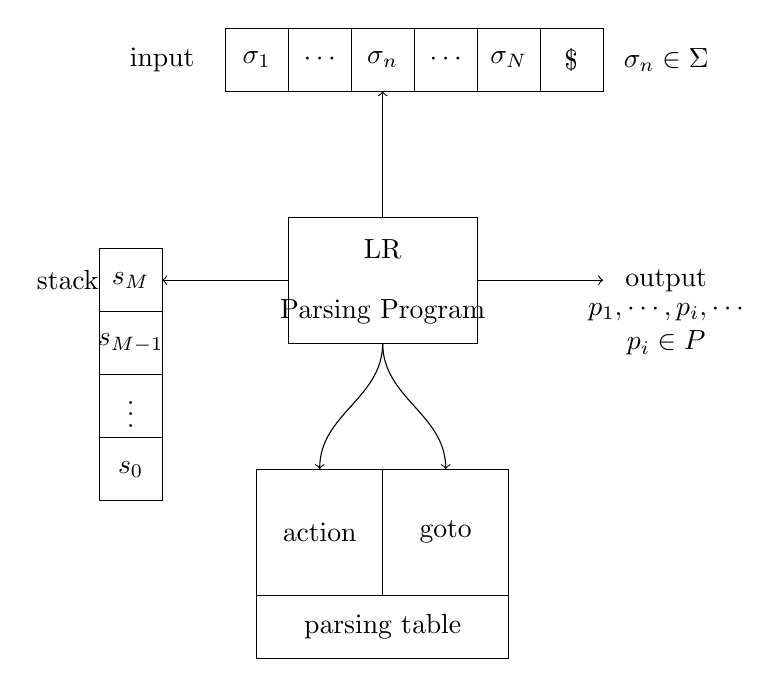
\begin{tikzpicture}
  [x=4mm,y=4mm,node distance=1,
    dati/.style={rounded corners,draw},
    box/.style={draw},
    stgrid/.style={draw=#1,},
    agrid/.style={stgrid=black!10},
    bgrid/.style={stgrid=cyan!50},
]

  \draw[box] (-3,-2)--(-3,2)--(3,2)--(3,-2)--cycle;
  \node(lr) at (0,1) {LR};
  \node(pp) at (0,-1) {Parsing Program};

  \draw[box] (-5,6)--(-3,6)--(-3,8)--(-5,8)--cycle;
  \draw[box] (-3,6)--(-1,6)--(-1,8)--(-3,8)--cycle;
  \draw[box] (-1,6)--( 1,6)--( 1,8)--(-1,8)--cycle;
  \draw[box] ( 1,6)--( 3,6)--( 3,8)--( 1,8)--cycle;
  \draw[box] ( 3,6)--( 5,6)--( 5,8)--( 3,8)--cycle;
  \draw[box] ( 5,6)--( 7,6)--( 7,8)--( 5,8)--cycle;

  \node(input) at (-7,7) {input};
  \node(a1) at (-4,7) {$\sigma_1$};
  \node(a2) at (-2,7) {$\cdots$};
  \node(a3) at ( 0,7) {$\sigma_n$};
  \node(a4) at ( 2,7) {$\cdots$};
  \node(a5) at ( 4,7) {$\sigma_N$};
  \node(a6) at ( 6,7) {\$};
  \node(an) at (9,7) {$\sigma_n\in \Sigma$};

  \node(output) at (9,0) {output};
  \node(output1) at (9,-1) {$p_1,\cdots,p_i,\cdots$};
  \node(output1) at (9,-2) {$p_i\in P$};
  
  \draw[->] (0,2)--(0,6);
  \draw[->] (3,0)--(7,0);
  \draw[->] (-3,0)--(-7,0);

  \draw[box] (-9,-1)--(-7,-1)--(-7,1)--(-9,1)--cycle;
  \draw[box] (-9,-3)--(-7,-3)--(-7,-1)--(-9,-1)--cycle;
  \draw[box] (-9,-5)--(-7,-5)--(-7,-3)--(-9,-3)--cycle;
  \draw[box] (-9,-7)--(-7,-7)--(-7,-5)--(-9,-5)--cycle;
  
  \node(sM) at (-8,0) {$s_M$};
  \node(sM1) at (-8,-2) {$s_{M-1}$};
  \node(sM2) at (-8,-4) {$\vdots$};
  \node(s0) at (-8,-6) {$s_0$};

  \node(stack) at (-10,0) {stack};

  \draw[box] (-4,-6)--(-4,-10)--(0,-10)--(0,-6)--cycle;
  \draw[box] (0,-6)--(0,-10)--(4,-10)--(4,-6)--cycle;
  \draw[box] (-4,-10)--(-4,-12)--(4,-12)--(4,-10)--cycle;
  
  \node(action) at (-2,-8) {action};
  \node(goto) at (2,-8) {goto};
  \node(pt) at (0,-11) {parsing table};

  \draw[->] (0,-2) to[out=270,in=90] (-2,-6);
  \draw[->] (0,-2) to[out=270,in=90] (2,-6);

\end{tikzpicture}
\end{scriptsize}

\vspace{1em}
\begin{scriptsize}
\begin{tabular}[t]{ll@{\hspace{1cm}}r|cccccc|ccc}
$p_1$ & E \spzbnf E + T &&\multicolumn{6}{c|}{\it action}
&\multicolumn{3}{c}{\it goto}\\
$p_2$ & E \spzbnf T &&\multicolumn{6}{c|}{(terminali)}
&\multicolumn{3}{c}{(non term.)}\\
$p_3$ & T \spzbnf T * F &{\it state} & a & + & * & ( & ) & \$ & E & T & F \\
\cline{3-12} 
$p_4$ & T \spzbnf F                  & 0  & $s_{5}$ &    &    & $s_{4}$ &     &           & $s_{1}$ & $s_{2}$ & $s_{3}$\\
$p_5$ & F \spzbnf ( E )              & 1  &    & $s_{6}$ &    &    &     & {\bf acc} &    &    & \\
$p_6$ & F \spzbnf a                  & 2  &    & $r_{2}$ & $s_{7}$ &    & $r_{2}$  & $r_{2}$        &    &    & \\
      &                        & 3  &    & $r_{4}$ & $r_{4}$ &    & $r_{4}$  & $r_{4}$        &    &    & \\
      & $\Sigma$=\{a,+,*,(,)\} & 4  & $s_{5}$ &    &    & $s_{4}$ &     &           & $s_{8}$ & $s_{2}$ & $s_{3}$\\
      & $V$=\{E,T,F\}          & 5  &    & $r_{6}$ & $r_{6}$ &    & $r_{6}$  & $r_{6}$        &    &    & \\
      & $S$=E                  & 6  & $s_{5}$ &    &    & $s_{4}$ &     &           &    & $s_{9}$ & $s_{3}$\\
      &                        & 7  & $s_{5}$ &    &    & $s_{4}$ &     &           &    &    & $s_{10}$\\
      &                        & 8  &    & $s_{6}$ &    &    & $s_{11}$ &           &    &    & \\
      &                        & 9  &    & $r_{1}$ & $s_{7}$ &    & $r_{1}$  & $r_{1}$        &    &    & \\
      &                        & 10 &    & $r_{3}$ & $r_{3}$ &    & $r_{3}$  & $r_{3}$        &    &    & \\
      &                        & 11 &    & $r_{5}$ & $r_{5}$ &    & $r_{5}$  & $r_{5}$        &    &    & \\
\end{tabular}
\end{scriptsize}
}{fig:parserlr}

Un parser LR è un parser bottom-up shift-reduce nonbacktracking,
schematizzato in \figura{fig:parserlr}, che utilizza una tabella ({\it
  tabella di parsing}) per identificare le transizioni di stato, dati
una coppia $(s_i,\sigma_j)$ di stati (righe) e simboli (colonne).

Esistono diversi algoritmi che consentono di generare la tabella di
parsing a partire dalla definizione della grammatica (per i quali si
rimanda a \spzcite[221-247]{ahosethiullman1986}), che differiscono tra
loro in base alla complessità e al numero di grammatiche in grado di
tradurre. Le tabelle generate, anche se sono diverse per la stessa
grammatica, hanno comunque la stessa struttura di
\figura{fig:parserlr}. A fronte di una coppia $(s_i,\sigma_j)$ ci
possono essere quattro azioni \spzcite[217-218]{ahosethiullman1986}:
\begin{enumerate}
\item {\it shift k ($s_k$)}: inserisce $s_i$ sullo stack, si posiziona
  dopo $\sigma_j$ e passa allo stato $s_k$;
\item {\it reduce n ($r_n$)}: dà in output la regola di produzione
  $p_n=v_h\spzmbnf t_1\cdots t_M$, toglie dallo stack $M$ stati, esponendo lo
  stato $s_l$; come stato, sceglie quello indicato da $(s_l,v_h)$
  (area {\it goto}) e rimane prima di $\sigma_j$;
\item {\it accept (acc)}: termina il parsing con successo;
\item {\it error (cella vuota)}: segnala un errore.
\end{enumerate}

Quello che bisogna definire quindi sono degli oggetti per le {\it
  azioni} e gli {\it stati}, e delle relazioni che associno i simboli
(terminali e no, ossia le classi di equivalenza e i sintagmi) con gli
stati e le azioni.

\newpage

\subsubsection{Parser LR con stack strutturato a grafo}

\tabula{Esempio di tabella di parsing per una grammatica ambigua}{tab:glr}{
\vspace{1em}
\begin{scriptsize}
\begin{tabular}[t]{r|cccccc|ccc}
&\multicolumn{6}{c|}{\it action}
&\multicolumn{3}{c}{\it goto}\\
&\multicolumn{6}{c|}{(terminali)}
&\multicolumn{3}{c}{(non term.)}\\
{\it state} & a & b & c & d & e & \$ & X & Y & Z \\
\hline
0  & $s_{5}$ &    &    & $s_{4}$ &     &           & $s_{1}$ & $s_{2}$ & $s_{3}$\\
1  &    & $s_{6}$ &    &    &     & {\bf acc} &    &    & \\
2  &    & $r_{2}$ & {\bf $s_{7}$,$r_6$} &    & $r_{2}$  & $r_{2}$        &    &    & \\
3  &    & $r_{4}$ & $r_{4}$ &    & $r_{4}$  & $r_{4}$        &    &    & \\
4  & $s_{5}$ &    &    & $s_{4}$ &     &           & $s_{8}$ & $s_{2}$ & $s_{3}$\\
5  &    & $r_{6}$ & $r_{6}$ &    & $r_{6}$  & $r_{6}$        &    &    & \\
6  & $s_{5}$ &    &    & {\bf $s_{4}$,$r_3$} &     &           &    & $s_{9}$ & $s_{3}$\\
7  & $s_{5}$ &    &    & $s_{4}$ &     &           &    &    & $s_{10}$\\
8  &    & $s_{6}$ &    &    & $s_{11}$ &           &    &    & \\
9  &    & $r_{1}$ & $s_{7}$ &    & $r_{1}$  & $r_{1}$        &    &    & \\
10 &    & $r_{3}$ & $r_{3}$ &    & $r_{3}$  & $r_{3}$        &    &    & \\
11 &    & $r_{5}$ & $r_{5}$ &    & $r_{5}$  & $r_{5}$        &    &    & \\
\end{tabular}
\end{scriptsize}
}

In \tabella{tab:glr} è riportato un esempio di tabella di parsing
ottenuta da una grammatica ambigua. Come si vede nelle celle
evidenziate, ci sono dei casi in cui una coppia stato-simbolo
$(s_i,\sigma_j)$ corrisponde a più azioni possibili. In questo caso un
parser LR standard fallirebbe.

Esiste un altro tipo di algoritmo, che procede normalmente come un
parser LR standard. Quando incontra una sequenza di azioni,
l'esecuzione viene suddivisa in più rami, ognuno dei quali procede in
parallelo finché non si raggiunge uno stato comune
\spzcitedue{}{tomita1985}{}{tomita1987}. È più semplice vederlo con
uno schema. L'algoritmo LR standard procede per passi successivi, con
un'azione per ogni passo, ad esempio:
\begin{lingeq}
\label{leq:lrstandard}
\begin{tikzpicture}[x=3mm,y=3mm,node distance=1]
\node(s0) {$\cdots$};
\node(s1) [right=of s0] {$s_{42}$};
\node(s2) [right=of s1] {$r_7$};
\node(s3) [right=of s2] {$s_{26}$};
\node(s4) [right=of s3] {$s_{33}$};
\node(s5) [right=of s4] {$r_{69}$};
\node(s6) [right=of s5] {$\cdots$};
\draw[->] (s0) to (s1);
\draw[->] (s1) to (s2);
\draw[->] (s2) to (s3);
\draw[->] (s3) to (s4);
\draw[->] (s4) to (s5);
\draw[->] (s5) to (s6);
\end{tikzpicture}
\end{lingeq}
\noindent mentre per il parser di Tomita l'esecuzione procede come
segue:
\begin{lingeq}
\label{leq:tlr}
\begin{tikzpicture}[x=3mm,y=3mm,node distance=1]
\node(s0) {$\cdots$};
\node(s1) [right=of s0] {$s_{42}$};
\node(s2) [right=of s1] {$s_7$};
\node(s3) [right=of s2] {$s_{26}$};
\node(s4) [right=of s3] {$r_{33}$};
\node(s5) [right=of s4] {$s_{69}$};
\node(s6) [right=of s5] {$s_{36}$};
\node(s7) [right=of s6] {$r_{74}$};
\node(s8) [right=of s7] {$\cdots$};
\node(s21) [below=of s2] {$r_{65}$};
\node(s31) [right=of s21] {$s_{88}$};
\node(s41) [right=of s31] {$s_{44}$};
\node(s42) [below=of s41] {$s_{69}$};
\node(s52) [right=of s42] {$r_{13}$};
\node(s71) [below=of s7] {$r_7$};
\node(s81) [right=of s71] {$\cdots$};

\draw[->] (s0) to (s1);
\draw[->] (s1) to (s2);
\draw[->] (s2) to (s3);
\draw[->] (s3) to (s4);
\draw[->] (s4) to (s5);
\draw[->] (s5) to (s6);
\draw[->] (s6) to (s7);
\draw[->] (s7) to (s8);

\draw[->] (s21) to (s31);
\draw[->] (s31) to (s41);
\draw[->] (s42) to (s52);

\draw[->] (s1) to (s21);
\draw[->] (s31) to (s4);
\draw[->] (s31) to (s42);
\draw[->] (s41) to (s5);
\draw[->] (s52) to (s6);
\draw[->] (s6) to (s71);
\end{tikzpicture}
\end{lingeq}

È chiaro quindi che con l'algoritmo indicato in \leqref{leq:tlr} è
possibile analizzare anche sequenze del tipo di quelle in
\tabella{tab:glr} e quindi permettere alla grammatica di essere
ambigua e di rilevare quest'ambiguità.

Per la strutturazione dei dati non cambia nulla: è sufficiente
prevedere che ogni coppia $(s_i,\sigma_j)$ possa essere associata a
più di un'azione.

\subsection{Lessico}

\begin{table}
\resizebox{\textwidth}{!}{\mbox{\begin{tabular}{|>{\it}r|r|*{8}{rr@{.}l@{\% }|}}
\hline
\multicolumn{1}{|c}{} & \multicolumn{1}{c|}{\it totale} &\multicolumn{3}{c|}{\it altro } & \multicolumn{3}{c|}{\it arabo } & \multicolumn{3}{c|}{\it cinese } & \multicolumn{3}{c|}{\it persiano } & \multicolumn{3}{c|}{\it arabo-persiano } & \multicolumn{3}{c|}{\it mediterraneo } & \multicolumn{3}{c|}{\it latino } & \multicolumn{3}{c|}{\it turco }\\
\hline
\hline
\multicolumn{26}{|c|}{\it grammaticali}\\
\hline
aggettivi pronominali & 2 & \multicolumn{3}{c|}{} & \multicolumn{3}{c|}{} & \multicolumn{3}{c|}{} & 1&50&00 & \multicolumn{3}{c|}{} & \multicolumn{3}{c|}{} & \multicolumn{3}{c|}{} & 1&50&00\\
 & 24 & \multicolumn{3}{c|}{} & \multicolumn{3}{c|}{} & \multicolumn{3}{c|}{} & 3&12&50 & \multicolumn{3}{c|}{} & \multicolumn{3}{c|}{} & \multicolumn{3}{c|}{} & 21&87&50\\
\hline
congiunzioni & 7 & \multicolumn{3}{c|}{} & 5&71&42 & \multicolumn{3}{c|}{} & 2&28&57 & \multicolumn{3}{c|}{} & \multicolumn{3}{c|}{} & \multicolumn{3}{c|}{} & \multicolumn{3}{c|}{}\\
 & 66 & \multicolumn{3}{c|}{} & 57&86&36 & \multicolumn{3}{c|}{} & 9&13&63 & \multicolumn{3}{c|}{} & \multicolumn{3}{c|}{} & \multicolumn{3}{c|}{} & \multicolumn{3}{c|}{}\\
\hline
numerali & 9 & \multicolumn{3}{c|}{} & \multicolumn{3}{c|}{} & \multicolumn{3}{c|}{} & \multicolumn{3}{c|}{} & \multicolumn{3}{c|}{} & \multicolumn{3}{c|}{} & \multicolumn{3}{c|}{} & 9&100&00\\
 & 15 & \multicolumn{3}{c|}{} & \multicolumn{3}{c|}{} & \multicolumn{3}{c|}{} & \multicolumn{3}{c|}{} & \multicolumn{3}{c|}{} & \multicolumn{3}{c|}{} & \multicolumn{3}{c|}{} & 15&100&00\\
\hline
post e preposizioni & 9 & \multicolumn{3}{c|}{} & 1&11&11 & \multicolumn{3}{c|}{} & \multicolumn{3}{c|}{} & \multicolumn{3}{c|}{} & \multicolumn{3}{c|}{} & \multicolumn{3}{c|}{} & 8&88&88\\
 & 20 & \multicolumn{3}{c|}{} & 1&5&00 & \multicolumn{3}{c|}{} & \multicolumn{3}{c|}{} & \multicolumn{3}{c|}{} & \multicolumn{3}{c|}{} & \multicolumn{3}{c|}{} & 19&95&00\\
\hline
pronomi & 4 & \multicolumn{3}{c|}{} & \multicolumn{3}{c|}{} & \multicolumn{3}{c|}{} & \multicolumn{3}{c|}{} & \multicolumn{3}{c|}{} & \multicolumn{3}{c|}{} & \multicolumn{3}{c|}{} & 4&100&00\\
 & 14 & \multicolumn{3}{c|}{} & \multicolumn{3}{c|}{} & \multicolumn{3}{c|}{} & \multicolumn{3}{c|}{} & \multicolumn{3}{c|}{} & \multicolumn{3}{c|}{} & \multicolumn{3}{c|}{} & 14&100&00\\
\hline
verbi ausiliari & 9 & \multicolumn{3}{c|}{} & \multicolumn{3}{c|}{} & \multicolumn{3}{c|}{} & \multicolumn{3}{c|}{} & \multicolumn{3}{c|}{} & \multicolumn{3}{c|}{} & \multicolumn{3}{c|}{} & 9&100&00\\
 & 72 & \multicolumn{3}{c|}{} & \multicolumn{3}{c|}{} & \multicolumn{3}{c|}{} & \multicolumn{3}{c|}{} & \multicolumn{3}{c|}{} & \multicolumn{3}{c|}{} & \multicolumn{3}{c|}{} & 72&100&00\\
\hline
\hline
tot. grammaticali & 40 & \multicolumn{3}{c|}{} & 6&15&00 & \multicolumn{3}{c|}{} & 3&7&50 & \multicolumn{3}{c|}{} & \multicolumn{3}{c|}{} & \multicolumn{3}{c|}{} & 31&77&50\\
 & 211 & \multicolumn{3}{c|}{} & 58&27&48 & \multicolumn{3}{c|}{} & 12&5&68 & \multicolumn{3}{c|}{} & \multicolumn{3}{c|}{} & \multicolumn{3}{c|}{} & 141&66&82\\
\hline
\hline
\multicolumn{26}{|c|}{\it lessico}\\
\hline
aggettivi & 54 & \multicolumn{3}{c|}{} & 41&75&92 & \multicolumn{3}{c|}{} & 12&22&22 & \multicolumn{3}{c|}{} & \multicolumn{3}{c|}{} & \multicolumn{3}{c|}{} & 1&1&85\\
 & 66 & \multicolumn{3}{c|}{} & 51&77&27 & \multicolumn{3}{c|}{} & 14&21&21 & \multicolumn{3}{c|}{} & \multicolumn{3}{c|}{} & \multicolumn{3}{c|}{} & 1&1&51\\
\hline
aggettivi comparativi & 1 & \multicolumn{3}{c|}{} & 1&100&00 & \multicolumn{3}{c|}{} & \multicolumn{3}{c|}{} & \multicolumn{3}{c|}{} & \multicolumn{3}{c|}{} & \multicolumn{3}{c|}{} & \multicolumn{3}{c|}{}\\
 & 2 & \multicolumn{3}{c|}{} & 2&100&00 & \multicolumn{3}{c|}{} & \multicolumn{3}{c|}{} & \multicolumn{3}{c|}{} & \multicolumn{3}{c|}{} & \multicolumn{3}{c|}{} & \multicolumn{3}{c|}{}\\
\hline
avverbi & 18 & \multicolumn{3}{c|}{} & 9&50&00 & \multicolumn{3}{c|}{} & 4&22&22 & \multicolumn{3}{c|}{} & \multicolumn{3}{c|}{} & \multicolumn{3}{c|}{} & 5&27&77\\
 & 23 & \multicolumn{3}{c|}{} & 10&43&47 & \multicolumn{3}{c|}{} & 5&21&73 & \multicolumn{3}{c|}{} & \multicolumn{3}{c|}{} & \multicolumn{3}{c|}{} & 8&34&78\\
\hline
interiezioni & 1 & \multicolumn{3}{c|}{} & 1&100&00 & \multicolumn{3}{c|}{} & \multicolumn{3}{c|}{} & \multicolumn{3}{c|}{} & \multicolumn{3}{c|}{} & \multicolumn{3}{c|}{} & \multicolumn{3}{c|}{}\\
 & 2 & \multicolumn{3}{c|}{} & 2&100&00 & \multicolumn{3}{c|}{} & \multicolumn{3}{c|}{} & \multicolumn{3}{c|}{} & \multicolumn{3}{c|}{} & \multicolumn{3}{c|}{} & \multicolumn{3}{c|}{}\\
\hline
nomi & 156 & 2&1&28 & 123&78&84 & 1&0&64 & 15&9&61 & 1&0&64 & 4&2&56 & 2&1&28 & 8&5&12\\
 & 254 & 3&1&18 & 196&77&16 & 1&0&39 & 29&11&41 & 1&0&39 & 7&2&75 & 7&2&75 & 10&3&93\\
\hline
stati costrutti & 1 & \multicolumn{3}{c|}{} & \multicolumn{3}{c|}{} & \multicolumn{3}{c|}{} & \multicolumn{3}{c|}{} & 1&100&00 & \multicolumn{3}{c|}{} & \multicolumn{3}{c|}{} & \multicolumn{3}{c|}{}\\
 & 1 & \multicolumn{3}{c|}{} & \multicolumn{3}{c|}{} & \multicolumn{3}{c|}{} & \multicolumn{3}{c|}{} & 1&100&00 & \multicolumn{3}{c|}{} & \multicolumn{3}{c|}{} & \multicolumn{3}{c|}{}\\
\hline
verbi & 11 & \multicolumn{3}{c|}{} & \multicolumn{3}{c|}{} & \multicolumn{3}{c|}{} & 1&9&09 & \multicolumn{3}{c|}{} & \multicolumn{3}{c|}{} & \multicolumn{3}{c|}{} & 10&90&90\\
 & 15 & \multicolumn{3}{c|}{} & \multicolumn{3}{c|}{} & \multicolumn{3}{c|}{} & 1&6&66 & \multicolumn{3}{c|}{} & \multicolumn{3}{c|}{} & \multicolumn{3}{c|}{} & 14&93&33\\
\hline
\hline
tot. lessico & 242 & 2&0&82 & 175&72&31 & 1&0&41 & 32&13&22 & 2&0&82 & 4&1&65 & 2&0&82 & 24&9&91\\
 & 363 & 3&0&82 & 261&71&90 & 1&0&27 & 49&13&49 & 2&0&55 & 7&1&92 & 7&1&92 & 33&9&09\\
\hline
\hline
altro & 1 & \multicolumn{3}{c|}{} & 1&100&00 & \multicolumn{3}{c|}{} & \multicolumn{3}{c|}{} & \multicolumn{3}{c|}{} & \multicolumn{3}{c|}{} & \multicolumn{3}{c|}{} & \multicolumn{3}{c|}{}\\
 & 1 & \multicolumn{3}{c|}{} & 1&100&00 & \multicolumn{3}{c|}{} & \multicolumn{3}{c|}{} & \multicolumn{3}{c|}{} & \multicolumn{3}{c|}{} & \multicolumn{3}{c|}{} & \multicolumn{3}{c|}{}\\
\hline
nomi propri & 9 & \multicolumn{3}{c|}{} & \multicolumn{3}{c|}{} & \multicolumn{3}{c|}{} & \multicolumn{3}{c|}{} & \multicolumn{3}{c|}{} & \multicolumn{3}{c|}{} & \multicolumn{3}{c|}{} & \multicolumn{3}{c|}{}\\
 & 17 & \multicolumn{3}{c|}{} & \multicolumn{3}{c|}{} & \multicolumn{3}{c|}{} & \multicolumn{3}{c|}{} & \multicolumn{3}{c|}{} & \multicolumn{3}{c|}{} & \multicolumn{3}{c|}{} & \multicolumn{3}{c|}{}\\
\hline
\hline
totale & 292 & 2&0&70 & 182&64&31 & 1&0&35 & 35&12&36 & 2&0&70 & 4&1&41 & 2&0&70 & 55&19&43\\
 & 592 & 3&0&52 & 320&55&65 & 1&0&17 & 61&10&60 & 2&0&34 & 7&1&21 & 7&1&21 & 174&30&26\\
\hline
\end{tabular}}}
\caption{Statistiche. In ogni cella, la prima riga rappresenta il numero di parole distinte, la seconda tiene conto anche delle ripetizioni.
        }
\label{tab:statistiche}
\end{table}

\afterpage{\clearpage}

Il lessico è forse la parte più importante del lavoro del filologo sui
documenti d'archivio: sia perché l'evoluzione diacronica del
linguaggio riguarda principalmente il lessico, sia perché è tramite il
lessico che ci si riallaccia allo studio storico sui documenti. In
questo senso, due sono le informazioni che è indispensabile
registrare:\footnote{Strettamente parlando, questo tipo di
  informazioni sarebbe necessario collezionarle anche per la
  grammatica. Ne parliamo solo qui per semplicità, ma è una cosa da
  tenere presente nei successivi sviluppi.}
\begin{itemize}
\item l'{\it etimologia} delle parole; (\vedi
  \tabella{tab:esempiostatistiche} come esempio di analisi);
\item le {\it note bibliografiche}, sia di attestazione dei termini,
  che di altre ricerche.
\end{itemize}

Visto che uno degli scopi è quello di generare un dizionario dei
termini di un insieme di documenti (\vedi \tabella{tab:esdiz}), è
opportuno registrare il significato (così come lo si trova nei normali
vocabolari) e altre annotazioni a discrezione dell'utente
(traslitterazioni, pronuncia, ecc.).

Oltre a questo, è necessario associare a ogni termine le informazioni
utili per l'analisi sintattica, sotto forma di caratteristiche
(transitivo, ditransitivo, collettivo, astratto, ecc.) e di tipo di
attributi richiesti. 

Infine, dal punto di vista più strettamente semantico, i temini
andrebbero categorizzati. Qui si possono usare vari modelli, che
possono associare caratteristiche a un certo termine oppure includere
il termine in un insieme \spzcite[28-33]{delmonte2008}. 

Si possono identificare due categorie di oggetti per ogni termine: uno
che riguarda la {\it forma} dell'oggetto (etimologia e altre
caratteristiche decise dall'utente) e uno che riguarda il {\it
  significato} (caratteristiche sintattiche, categorizzazione, ecc.).

In entrambi i casi, i dati possono essere strutturati in più modi, per
esempio:
\begin{itemize}
\item tramite descrizioni (in modo analogo a quanto fatto nella parte
  morfologica);
\item tramite associazioni dirette tra due termini (nel caso di
  un'antinomia per esempio);
\item tramite inclusione di termini in insiemi di termini collegati
  (sul modello di FrameNet).
\end{itemize}

L'organizzazione di questi dati dipende molto dal tipo di ricerca: è
quindi opportuno dare all'utente più metodi di lavoro possibili. È
necessario però prevedere delle tabelle derivate dove le diverse
classificazioni vengano tradotte in una forma consona all'analisi
sintattica (\vedi \sezione{sec:conssintassi}).

\tabula{Esempio di voci del dizionario generato dal database lessicale
  del documento \spzcite{dt1099}, dove vengono registrate informazioni
  morfologiche, traslitterazioni, etimologie, significato e note
  bibliografiche divise in pronuncia e riferimenti
  generali. Abbreviazioni: n.=nome, a.=arabo.}  {tab:esdiz}{\vspace{-1em}\begin{glossario}{}
\item[\spzrl{istifsAr},] {\sf istifsar},\ n.\ a.:\ inchiesta, azione di fare domande; informazione.
\begin{subvocedue}
\item[Pron.:] \spzcite{redhouse1997}, \spzcite[192]{meninski1680d1}
\item[Rif.:] \spzcite[35]{kiefferbianchi18351}
\end{subvocedue}
\item[\spzrl{i.zhAr},] {\sf äzher},\ n.\ a.:\ manifestazione, esposizione, testimonianza.
\begin{subvocedue}
\item[Pron.:] \spzcite{redhouse1997}, \spzcite[275]{meninski1680d1}
\item[Rif.:] \spzcite[56]{kiefferbianchi18351}
\end{subvocedue}
\end{glossario}}

\section{Tabelle di base}
\label{sec:tabbase}

\subsection{Parsing preliminare}
\label{sec:parsing}

Come abbiamo visto in \sezione{sec:struttura}, è necessario definire
come suddividere il testo in modo che ogni token ottenuto rappresenti
una parola (nel senso comune del termine). Il metodo scelto prevede
l'uso di espressioni regolari, ognuna delle quali individua un tipo di
token, come scelto dall'utente.

\myfig[t]{Tabelle di base: definizione di lingua e espressioni
  regolari per il parsing iniziale. Le frecce indicano una foreign
  key (f.k.). In grigio le tabelle di relazione per le relazioni
  molti a molti.}{\begin{scriptsize}
\begin{tikzpicture}
  [x=5mm,y=5mm,node distance=0,
    %>=triangle 45,
    stgrid/.style={draw=#1!10,},
    agrid/.style={stgrid=black},
    bgrid/.style={stgrid=cyan},
    anchortab/.style={circle,draw},
    tab/.style={rounded corners,
      top color=white, 
      bottom color=#1!20,
    },
    tabtop/.style={rounded corners,
      top color=#1!5, 
      bottom color=#1,
    },
    tabsoft/.style={rounded corners,
      top color=white, 
      bottom color=#1!5,
    },
    tabsofttop/.style={rounded corners,
      top color=#1!5, 
      bottom color=#1!25,
    },
    multirel/.style={tab=gray},
    multireltop/.style={tabtop=gray},
    alpha/.style={tab=green},
    alphatop/.style={tabtop=green},
    morph/.style={tab=blue},
    morphtop/.style={tabtop=blue},
    syntax/.style={tab=yellow},
    syntaxtop/.style={tabtop=yellow},
    lexicon/.style={tab=red},
    lexicontop/.style={tabtop=red},
  ]

  \begin{dbtabella}{alpha}{0}{3}{8}{1}{\alphapref}{tokenregexpset}
    \tablerow{name}{varchar(1024)}
  \end{dbtabella}

  \begin{dbtabella}{alpha}{0}{-8}{8}{2}{\alphapref}{tokenregexp}
    \tablerow{name}{varchar(1024)}
    \tablerow{regexp}{varchar(1024)}
  \end{dbtabella}

  \begin{dbtabella}{multirel}{2}{-1}{9}{4}{\alphapref}{tokenregexpsetthrough}
    \tablerow{order}{integer}
    \tablerow{disabled}{boolean}
    \tablelink[left]{token regexp set}{tokenregexpset}
    \tablelink[left]{token regexp}{tokenregexp}
  \end{dbtabella}

  \begin{dbtabella}{alpha}{-15}{5}{9}{3}{\alphapref}{language}
    \tablerow{name}{varchar(1024)}
    \tablelink{token regexp set}{tokenregexpset}
    \tablelink{period sep}{tokenregexp}
  \end{dbtabella}
\end{tikzpicture}
\end{scriptsize}
}{fig:alpha}

In \figura{fig:alpha} sono rappresentate le tabelle necessarie. Una
lingua è definita da un insieme di espressioni regolari. Di queste,
una viene scelta per definire i delimitatori di periodo: è necessario
imporre un vincolo, in modo che il delimitatore di periodo sia tra i
token previsti per la lingua.\footnote{Il modo in cui imporre questo
  vincolo dipende dal motore di database e dall'applicazione. In
  Django è sufficiente definire un controllo aggiuntivo in fase di
  salvataggio dei dati. Volendo, con PostgreSQL si può definire un
  trigger, ossia un controllo che viene eseguito al momento
  dell'inserimento dei dati. Altri motori possono usare altri
  meccanismi.} Il delimitatore di periodo individua quei token che
fanno fermare l'analizzatore sintattico (una funzione equivalente a
quella del simbolo \$ in \figura{fig:parserlr}).

\tabula[p]{Esempio di espressioni regolari per il parsing
  dell'italiano, in grassetto quella possibile come separatore di
  periodi. Nella tabella in basso l'output risultante con un brano di
  esempio. Le notazioni {\tt (?={\it x})}, {\tt (?!{\it x})}, {\tt
    (?<={\it x})} e {\tt (?<!{\it x})} sono estensioni di Python
  (individuano il testo adiacente, rispettivamente come seguito, non
  seguito, preceduto, non preceduto da {\it x}). }{tab:alpha}{
\noindent\begin{scriptsize}
\begin{tabular}{l>{\tt}l>{\it}p{3cm}}
space            & [ ] & spazio da solo\\
dialog mark      & [\textquotedbl «»“”]\\
hyphen           & [—-] & tipi diversi di trattino\\
ellipses         & …|[.]\{2,\} & tre puntini (unico carattere) o più di due punti consecutivi\\
numbers          & [0-9]+\\
brackets         & [()\{\}\textbackslash [\textbackslash ]]\\
apostrophe alone & (?<![a-zA-ZàèìòùáéíóúÀÈÌÒÙÁÉÍÓÚ])[\textquotesingle ’]&apostrofo non preceduto da altri caratteri\\
alpha            & [a-zA-ZàèìòùáéíóúÀÈÌÒÙÁÉÍÓÚ]+[\textquotesingle ’]?&caratteri alfabetici eventualmente seguiti da apostrofo\\
others           & [\^{}()\{\}\textbackslash [\textbackslash ]a-zA-ZàèìòùáéíóúÀÈÌÒÙÁÉÍÓÚ ?,;:!….\textquotesingle ’\textbackslash t\textbackslash n\textbackslash r0-9\textquotedbl«»“”—-]&caratteri che non sono quelli dell'elenco\\
tab              & [\textbackslash t]\\
new line         & [\textbackslash n\textbackslash r]\\
{\bf period}     & (?<![.])[.](?![.])|[?;:!]&punto isolato o altri segni di interpunzione forte\\
punctuation mark & [,]\\
\end{tabular}
\vspace{1em}

\begin{tabular}[h]{|*{10}{l|}}
\hline
Un& &raggio& &di& &sole& &filtrò& \\
{\it alpha}&{\it space}&{\it alpha}&{\it space}&{\it alpha}&{\it space}&{\it alpha}&{\it space}&{\it alpha}&{\it space}\\
\hline
con& &decisione& &dalla& &finestra&,& &invase\\
{\it alpha}&{\it space}&{\it alpha}&{\it space}&{\it alpha}&{\it space}&{\it alpha}&{\it p. mark}&{\it space}&{\it alpha}\\
\hline
 &la& &camera& &783& &dell’&hotel& \\
{\it space}&{\it alpha}&{\it space}&{\it alpha}&{\it space}&{\it numbers}&{\it space}&{\it alpha}&{\it alpha}&{\it space}\\
\hline
e& &si& &andò& &a& &schiantare&,\\
{\it alpha}&{\it space}&{\it alpha}&{\it space}&{\it alpha}&{\it space}&{\it alpha}&{\it space}&{\it alpha}&{\it p. mark}\\
\hline
 &dritto& &dritto&,& &sul& &suo& \\
{\it space}&{\it alpha}&{\it space}&{\it alpha}&{\it p. mark}&{\it space}&{\it alpha}&{\it space}&{\it alpha}&{\it space}\\
\hline
occhio& &sinistro&.& &“&Oh& &no&,\\
{\it alpha}&{\it space}&{\it alpha}&{\it period}&{\it space}&{\it d. mark}&{\it alpha}&{\it space}&{\it alpha}&{\it p. mark}\\
\hline
”& &pensò& &Roberto& &deciso& &a& \\
{\it d. mark}&{\it space}&{\it alpha}&{\it space}&{\it alpha}&{\it space}&{\it alpha}&{\it space}&{\it alpha}&{\it space}\\
\hline
non& &arrendersi&,& &“&sono& &stanco&,\\
{\it alpha}&{\it space}&{\it alpha}&{\it p. mark}&{\it space}&{\it d. mark}&{\it alpha}&{\it space}&{\it alpha}&{\it p. mark}\\
\hline
 &voglio& &dormire& &ancora&.&”\\
{\it space}&{\it alpha}&{\it space}&{\it alpha}&{\it space}&{\it alpha}&{\it period}&{\it d. mark}\\
\hline
\end{tabular}
\end{scriptsize}
}

\afterpage{\clearpage}

In \tabella{tab:alpha} è riportato un esempio di come possono essere
definite delle regole di parsing per un testo in italiano corrente. Le
espressioni regolari sono un formalismo molto potente, che consentono
di suddividere un brano con un'unica operazione e una precisione
definibile a piacere. Nella versione più semplice, l'applicazione
concatena tutte le espressioni regolari definite dall'utente, aggiunge
quelle per i tag di formattazione e utilizza l'espressione risultante
per suddividere il testo. Quindi confronta i token ottenuti con
l'elenco delle espressioni regolari per etichettarli.\footnote{Il
  metodo reale di parsing e la descrizione dell'espressione regolare
  dipendono dal linguaggio di programmazione scelto. Qui e in seguito
  si userà quanto stabilito dalla libreria {\it re} di Python
  \spzcitedue{}{pythonre}{}{kuchling2012}. Per una trattazione più
  generale si veda \spzcite{cinderella1979}.}

Quindi per esempio, definite le espressioni regolari:

\begin{lingtab}{l>{\tt}l}
\label{leq:itregexp}
alpha & [a-z]+\\
space & [ ]\\
numbers & [0-9]+\\
\end{lingtab}
\noindent l'espressione regolare risultante diventa:
\begin{lingeq}
{\tt ([a-z]+|[ ]|[0-9]+) }
\end{lingeq}
\noindent e utilizzando una funzione di split per espressioni regolari, la frase
{\it oggi ho letto 3 libri} viene suddivisa in 
\begin{lingeq}
{\tt [ `oggi' , ` ' , `ho' , ' ' , `letto' , ` ' , `3' , ` ' , `libri' ]}. 
\end{lingeq}

A questo punto un successivo confronto indivduerà `3' come un token di
tipo {\it numbers}, `oggi', `ho', `letto' e `libri' come token di tipo
{\it alpha} e gli altri come token di tipo {\it space}.

Da notare che con le espressioni regolari definite in
\leqref{leq:itregexp}, la frase {\it oggi, come di consuento, ho letto
  3 libri}, produce un token aggiuntivo, `,', che verrà marcato come
       {\it sconosciuto} in quanto non previsto da nessuna
       regola.\footnote{La funzione di split, qui considerata come
         esempio di metodo di parsing, suddivide una stringa basandosi
         su un'espressione regolare data come delimitatore.  Ossia,
         data l'espressione regolare {\tt a+}, suddivide la stringa
         {\it defaabaghj} in {\tt ['def','b','ghj']}. Se si usano le
         parentesi, ossia {\tt (a+)}, ritorna anche le occorrenze
         della stringa, ossia: {\tt ['def','aa','b','a','ghj']}, che è
         il risultato che ci interessa \spzcite{pythonre}. } L'utente
       dovrà quindi inserire una nuova espressione regolare, per esempio:
\begin{lingtab}{l>{\tt}l}
punctuation & [.:;,?!]\\
\end{lingtab}
\noindent che consente al programma di individuare il tipo giusto per il token `,'.

\subsection{Descrizioni}

\label{sec:descrdb}

\myfig[t]{Tabelle di base: descrizioni. Le frecce indicano una foreign
  key (f.k.). In grigio le tabelle di relazione per le relazioni molti
  a molti. Una descrizione è una collezione di coppie attributo/valore
  o attributo/descrizione: quindi viene rappresentata come una tabella
  ({\it description}) con due relazioni molti a molti, rispettivamente
  con una tabella che unisce attributi e valori ({\it entry}) e una
  tabella che unisce attributi e descrizioni ({\it subdescription}). I
  valori (tabella {\it value}) possono essere costanti (campo {\it
    variable} posto a `false') o variabili (campo {\it variable} posto
  a `true'). All'interno di una descrizione possono apparire anche
  come negati (campo {\it negate} della tabella {\it
    entry}).}{\begin{scriptsize}
\begin{tikzpicture}
  [x=5mm,y=5mm,node distance=0,
    %>=triangle 45,
    stgrid/.style={draw=#1!10,},
    agrid/.style={stgrid=black},
    bgrid/.style={stgrid=cyan},
    anchortab/.style={circle,draw},
    tab/.style={rounded corners,
      top color=white, 
      bottom color=#1!20,
    },
    tabtop/.style={rounded corners,
      top color=#1!5, 
      bottom color=#1,
    },
    tabsoft/.style={rounded corners,
      top color=white, 
      bottom color=#1!5,
    },
    tabsofttop/.style={rounded corners,
      top color=#1!5, 
      bottom color=#1!25,
    },
    multirel/.style={tab=gray},
    multireltop/.style={tabtop=gray},
    alpha/.style={tab=green},
    alphatop/.style={tabtop=green},
    morph/.style={tab=blue},
    morphtop/.style={tabtop=blue},
    syntax/.style={tab=yellow},
    syntaxtop/.style={tabtop=yellow},
    lexicon/.style={tab=red},
    lexicontop/.style={tabtop=red},
  ]

  \begin{dbtabella}{alpha}{11}{9}{7}{1}{\alphapref}{attribute}
    \tablerow{name}{varchar(1024)}
  \end{dbtabella}

  \begin{dbtabella}{alpha}{11}{-4}{7}{2}{\alphapref}{value}
    \tablerow{string}{varchar(1024)}
    \tablerow{variable}{boolean}
  \end{dbtabella}

  \begin{dbtabella}{alpha}{2}{3}{7}{1}{\alphapref}{description}
    \tablerow{name}{varchar(1024)}
  \end{dbtabella}

  \begin{dbtabella}{alpha}{3}{-2}{6}{3}{\alphapref}{entry}
    \tablelink{attribute}{attribute}
    \tablelink{value}{value}
    \tablerow{negate}{boolean}
  \end{dbtabella}

  \begin{dbtabella}{multirel}{-7}{0}{7}{2}{\alphapref}{}
    \tablelink{description}{description}
    \tablelink{entry}{entry}
  \end{dbtabella}

  \begin{dbtabella}{alpha}{-7}{10}{7}{2}{\alphapref}{subdescription}
    \tablelink{attribute}{attribute}
    \tablelink{description}{description}
  \end{dbtabella}

  \begin{dbtabella}{multirel}{-8}{5}{8}{2}{\alphapref}{}
    \tablelink[left]{subdescription}{subdescription}
    \tablelink{description}{description}
  \end{dbtabella}

\end{tikzpicture}
\end{scriptsize}
}{fig:description}

La rappresentazione di una descrizione (\vedi
\sezione{sec:descrizioni}) nel database è riportata in
\figura{fig:description}. Una descrizione è una collezione di coppie
attributo/valore o attributo/descrizione: quindi viene rappresentata
come una tabella ({\it description}) con due relazioni molti a molti,
rispettivamente con una tabella che unisce attributi e valori ({\it
  entry}) e una tabella che unisce attributi e descrizioni ({\it
  subdescription}). I valori (tabella {\it value}) possono essere
costanti (campo {\it variable} posto a `false') o variabili (campo
{\it variable} posto a `true'). All'interno di una descrizione possono
apparire anche come negati (campo {\it negate} della tabella {\it
  entry}).

\section{Tabelle morfologiche}

\label{sec:temimorph}

Anche in questo caso, come meccanismo base abbiamo usato le
espressioni regolari, elencate nella tabella delle sostituzioni (\vedi
\figura{fig:regexpreplacement}).\label{page:regexpreplacement} Ogni
sostituzione è definita da due campi, un'espressione regolare ({\it
  pattern}) e la stringa che definisce la sostituzione ({\it
  replacement}).

\myfig{Morfologia: sostituzioni basate su espressioni
  regolari. A lato degli esempi.}{\begin{scriptsize}
\begin{tikzpicture}
  [x=5mm,y=5mm,node distance=0,
    %>=triangle 45,
    stgrid/.style={draw=#1!10,},
    agrid/.style={stgrid=black},
    bgrid/.style={stgrid=cyan},
    anchortab/.style={circle,draw},
    tab/.style={rounded corners,
      top color=white, 
      bottom color=#1!20,
    },
    tabtop/.style={rounded corners,
      top color=#1!5, 
      bottom color=#1,
    },
    tabsoft/.style={rounded corners,
      top color=white, 
      bottom color=#1!5,
    },
    tabsofttop/.style={rounded corners,
      top color=#1!5, 
      bottom color=#1!25,
    },
    multirel/.style={tab=gray},
    multireltop/.style={tabtop=gray},
    alpha/.style={tab=green},
    alphatop/.style={tabtop=green},
    morph/.style={tab=blue},
    morphtop/.style={tabtop=blue},
    syntax/.style={tab=yellow},
    syntaxtop/.style={tabtop=yellow},
    lexicon/.style={tab=red},
    lexicontop/.style={tabtop=red},
  ]

  \begin{dbtabella}{morph}{20}{25}{10}{2}{morphology}{regexpreplacement}
    \tablerow{pattern}{varchar(1024)}
    \tablerow{replacement}{varchar(1024)}
  \end{dbtabella}

\end{tikzpicture}
\end{scriptsize}

\noindent\begin{scriptsize}
\begin{tabular}[b]{*{2}{>{\tt}l}lll}
\multicolumn{1}{l}{\it pattern}&
\multicolumn{1}{l}{\it replacement}\\
(.*) & \textbackslash 1iamo & (am) & (am)iamo & amiamo\\
(.*)([bcdfglmnpqrstvz]) &\textbackslash 1\textbackslash 2\textbackslash 2ia
& (sa)(p) & (sa)(p)(p)ia  & sappia\\
\end{tabular}
\end{scriptsize}
}{fig:regexpreplacement}

Una radice tematica è l'unione di una radice lessicale e di una regola
di derivazione, mentre una parola è l'unione di una radice tematica
con una regola di flessione (per la composizione vedi
\sezione{sec:composizione}). Per rappresentarle sono sufficienti tre
tabelle, quella delle radici lessicali ({\it root}), quella delle
regole di derivazione ({\it derivation}) e quella delle regole di
flessione ({\it inflection}): le tabelle delle radici tematiche ({\it
  stem}) e delle parole ({\it word}) possono essere calcolate in base
alle caratteristiche delle altre tre. Per questioni di prestazione, è
prevista anche una tabella di cache ({\it wordcache}), che è quella
usata dalla componente di analisi dei testi.

\myfig{Morfologia: relazioni tra radici lessicali ({\it root}), radici
  tematiche ({\it stem}) e parole ({\it word}). In colore più chiaro
  le tabelle calcolate.}{\begin{scriptsize}
\begin{tikzpicture}
  [x=5mm,y=5mm,node distance=0,
    %>=triangle 45,
    stgrid/.style={draw=#1,},
    agrid/.style={stgrid=black!10},
    bgrid/.style={stgrid=cyan!50},
    anchortab/.style={circle,draw},
    tab/.style={rounded corners,
      top color=white, 
      bottom color=#1!20,
    },
    tabtop/.style={rounded corners,
      top color=#1!5, 
      bottom color=#1,
    },
    tabsoft/.style={rounded corners,
      top color=white, 
      bottom color=#1!5,
    },
    tabsofttop/.style={rounded corners,
      top color=#1!5, 
      bottom color=#1!25,
    },
    multirel/.style={tab=gray},
    multireltop/.style={tabtop=gray},
    alpha/.style={tab=green},
    alphatop/.style={tabtop=green},
    morph/.style={tab=blue},
    morphtop/.style={tabtop=blue},
    morphcalc/.style={tab=bluea},
    morphcalctop/.style={tabtop=bluea},
    morphcache/.style={tab=blueb},
    morphcachetop/.style={tabtop=blueb},
    syntax/.style={tab=yellow},
    syntaxtop/.style={tabtop=yellow},
    lexicon/.style={tab=red},
    lexicontop/.style={tabtop=red},
  ]

  \begin{dbtabella}{morph}{9}{20}{11}{5}{morphology}{root}
    \tablerow{root}{varchar(1024)}
    \tablerow{language}{f.k. language}
    \tablerow{description}{f.k. description}
    \tablerow{tema}{f.k. tema}
    \tablerow{part of speech}{f.k. partofspeech}
  \end{dbtabella}

  \begin{dbtabella}{morph}{9}{12}{12}{7}{morphology}{derivation}
    \tablerow{name}{varchar(1024)}
    \tableflink{regexp}{regexpreplacement}
    \tableflink{tema}{tema}
    \tableflink{description}{description}
    \tableflink{root description}{description}
    \tableflink{root part of speech}{partofspeech}
    \tableflink{paradigma}{paradigma}
  \end{dbtabella}

  \begin{dbtabella}{morphcalc}{0}{14}{7}{2}{morphology}{stem}
    \tablelink{root}{root}
    \tablelink{derivation}{derivation}
  \end{dbtabella}

  \begin{dbtabella}{morph}{9}{2}{10}{3}{morphology}{inflection}
    \tablerow{dict entry}{boolean}
    \tableflink{description}{description}
    \tableflink{regexp}{regexpreplacement}
  \end{dbtabella}

  \begin{dbtabella}{morphcalc}{-9}{10}{7}{2}{morphology}{word}
    \tablelink{stem}{stem}
    \tablelink{inflection}{inflection}
  \end{dbtabella}

  \begin{dbtabella}{morphcalc}{-7}{5}{7}{2}{morphology}{wordcache}
    \tableolink[left]{word}{word}
    \tablerow{cache}{cache}
  \end{dbtabella}

\end{tikzpicture}
\end{scriptsize}
}{fig:words}

Una tabella a parte è quella delle non-parole ({\it notword}), ossia
un elenco di token che non devono essere analizzati
morfologicamente. Questa tabella comprende spazi, tabulazioni, a capo,
punteggiatura, ecc. (\vedi \figura{fig:notword}).

\myfig[t]{Morfologia: non-parole. A lato degli esempi.}{\begin{scriptsize}
\begin{tabular}[b]{l>{\tt}l}
spazio & \\
punto & . \\
punto interrogativo & ?\\
virgola & ,\\
new line & \textbackslash n\\
\end{tabular}
\end{scriptsize} \begin{scriptsize}
\begin{tikzpicture}
  [x=5mm,y=5mm,node distance=0,
    %>=triangle 45,
    stgrid/.style={draw=#1!10,},
    agrid/.style={stgrid=black},
    bgrid/.style={stgrid=cyan},
    anchortab/.style={circle,draw},
    tab/.style={rounded corners,
      top color=white, 
      bottom color=#1!20,
    },
    tabtop/.style={rounded corners,
      top color=#1!5, 
      bottom color=#1,
    },
    tabsoft/.style={rounded corners,
      top color=white, 
      bottom color=#1!5,
    },
    tabsofttop/.style={rounded corners,
      top color=#1!5, 
      bottom color=#1!25,
    },
    multirel/.style={tab=gray},
    multireltop/.style={tabtop=gray},
    alpha/.style={tab=green},
    alphatop/.style={tabtop=green},
    morph/.style={tab=blue},
    morphtop/.style={tabtop=blue},
    syntax/.style={tab=yellow},
    syntaxtop/.style={tabtop=yellow},
    lexicon/.style={tab=red},
    lexicontop/.style={tabtop=red},
  ]

  \begin{dbtabella}{alpha}{11}{-3}{12}{3}{\alphapref}{language}
    \tablerow{name}{varchar(1024)}
    \tablerow{period sep}{f.k. tokenregexp}
    \tablerow{token regexp set}{f.k. tokenregexpset}
  \end{dbtabella}

  \begin{dbtabella}{morph}{0}{0}{9}{3}{morphology}{notword}
    \tablerow{name}{varchar(1024)}
    \tablerow{word}{varchar(1024)}
    \tablelink{language}{language}
  \end{dbtabella}


\end{tikzpicture}
\end{scriptsize}
}{fig:notword}

\subsection{Derivazione}

\label{sec:derivazione}

\myfig{Morfologia: radici.}{\begin{scriptsize}
\begin{tikzpicture}
  [x=5mm,y=5mm,node distance=0,
    %>=triangle 45,
    stgrid/.style={draw=#1,},
    agrid/.style={stgrid=black!10},
    bgrid/.style={stgrid=cyan!50},
    anchortab/.style={circle,draw},
    tab/.style={rounded corners,
      top color=white, 
      bottom color=#1!20,
    },
    tabtop/.style={rounded corners,
      top color=#1!5, 
      bottom color=#1,
    },
    tabsoft/.style={rounded corners,
      top color=white, 
      bottom color=#1!5,
    },
    tabsofttop/.style={rounded corners,
      top color=#1!5, 
      bottom color=#1!25,
    },
    multirel/.style={tab=gray},
    multireltop/.style={tabtop=gray},
    alpha/.style={tab=green},
    alphatop/.style={tabtop=green},
    morph/.style={tab=blue},
    morphtop/.style={tabtop=blue},
    morphcalc/.style={tab=bluea},
    morphcalctop/.style={tabtop=bluea},
    morphcache/.style={tab=blueb},
    morphcachetop/.style={tabtop=blueb},
    syntax/.style={tab=yellow},
    syntaxtop/.style={tabtop=yellow},
    lexicon/.style={tab=red},
    lexicontop/.style={tabtop=red},
  ]

  \begin{dbtabella}{alpha}{20}{15}{9}{1}{\alphapref}{description}
    \tablerow{name}{varchar(1024)}
  \end{dbtabella}

  \begin{dbtabella}{morph}{20}{11}{8}{1}{\alphapref}{partofspeech}
    \tablerow{name}{varchar(1024)}
  \end{dbtabella}

  \begin{dbtabella}{morph}{32}{18}{8}{1}{\alphapref}{temavalue}
    \tablerow{name}{varchar(1024)}
  \end{dbtabella}

  \begin{dbtabella}{morph}{32}{24}{8}{1}{\alphapref}{temaargument}
    \tablerow{name}{varchar(1024)}
  \end{dbtabella}
  
  \begin{dbtabella}{morph}{20}{20}{8}{1}{\alphapref}{tema}
    \tablerow{name}{varchar(1024)}
  \end{dbtabella}

  \begin{dbtabella}{multirel}{22}{26}{8}{3}{\alphapref}{}
    \tablelink[left]{tema}{tema}
    \tablelink{tema argument}{temaargument}
    \tablelink{tema value}{temavalue}
  \end{dbtabella}

  \begin{dbtabella}{morph}{9}{19}{9}{5}{morphology}{root}
    \tablerow{root}{varchar(1024)}
    \tableflink{language}{language}
    \tablelink{tema}{tema}
    \tablelink{description}{description}
    \tablelink{part of speech}{partofspeech}
  \end{dbtabella}


\end{tikzpicture}
\end{scriptsize}
}{fig:root}

Perché una regola di derivazione $d$ e una radice lessicale $r$
possano dar vita a una radice tematica $s$ devono essere compatibili,
ossia dev'essere possibile applicare $d$ a $r$. Le caratteristiche che
definiscono la compatibilità sono state divise in tre parti: la
categoria (verbale, nominale, ecc.), il tema e la descrizione della
radice.

La categoria di $r$, $r.{pos}$, è definita dal campo {\it part of
  speech} e dev'essere uguale al campo {\it root part of speech} di
$d$, $d.{rpos}$:
\begin{lingmeq}
r.{pos} = d.{rpos}\,.
\end{lingmeq}

Entrambi sono un collegamento alla tabella {\it partofspeech}, dove
l'utente definisce le parti del discorso che gli interessano.

Il tema è una versione semplificata di descrizione, dove gli attributi
possono essere associati solo a valori costanti e rappresentano tipi
di derivazioni possibili (\vedi \figura{fig:root}). Perché il tema di
$r$, $r.tema$, sia compatibile con quello di $d$, $d.tema$, bisogna
che:
\begin{lingmeq}
d.tema\spzmsussunto r.tema\,. 
\end{lingmeq}

Ad esempio, il tema della radice lessicale `\spzradless{bell}'
può essere descritto come:
\begin{lingmeq}
\left[\begin{array}{lll}
\text{base}&=&\text{-o}\\
\text{nome di qualità}&=&\text{-ezza}\\
\end{array}\right]
\end{lingmeq}
\noindent mentre quello di `\spzradless{amic}':
\begin{lingmeq}
\left[\begin{array}{lll}
\text{base}&=&\text{-o}\\
\text{nome di qualità}&=&\text{-izia}\\
\end{array}\right]
\end{lingmeq}

La regola di derivazione che ricava le radici tematiche
`\spzradtema{bell}' e `\spzradtema{amic}', avrà come tema:
\begin{lingmeq}
\left[\begin{array}{lll}
\text{base}&=&\text{-o}\\
\end{array}\right]
\end{lingmeq}
\noindent mentre quella che ricava `\spzradtema{bellezz}' avrà:
\begin{lingmeq}
\left[\begin{array}{lll}
\text{nome di qualità}&=&\text{-ezza}\\
\end{array}\right]
\end{lingmeq}
\noindent e quella che ricava `\spzradtema{amicizi}':
\begin{lingmeq}
\left[\begin{array}{lll}
\text{nome di qualità}&=&\text{-izia}\\
\end{array}\right]
\end{lingmeq}

Infine è necessario che la descrizione di $r$, $r.desc$, sussuma
quella richiesta per la radice da $d$, $d.{rdesc}$ (campo {\it root
  description}):
\begin{lingmeq}
d.{rdesc}\spzmsussunto r.desc\,. 
\end{lingmeq}

Ad esempio, se la radice lessicale `\spzradless{poet}' ha i seguenti parametri:
\begin{lingmeq}
\left\{\begin{array}{lll}
\text{categoria} & = & \text{nome} \\
\text{tema} & = &
\left[\begin{array}{lll}
\text{base}&=&\text{-a}\\
\text{femminile}&=&\text{-essa}\\
\end{array}\right]\\
\text{descrizione} & = &
\left[\begin{array}{lll}
\text{genere}&=&\text{maschile}\\
\end{array}\right]\\
\end{array}\right\}
\end{lingmeq}
\noindent è compatibile con i seguenti parametri di una
derivazione che genera nomi maschili in -a:
\begin{lingmeq}
\left\{\begin{array}{lll}
\text{categoria della radice} & = & \text{nome} \\
\text{tema} & = &
\left[\begin{array}{lll}
\text{base}&=&\text{-a}\\
\end{array}\right]\\
\text{descrizione della radice} & = &
\left[\begin{array}{lll}
\text{genere}&=&\text{maschile}\\
\end{array}\right]\\
\end{array}\right\}
\end{lingmeq}
\noindent o con i seguenti parametri di una
derivazione che genera nomi femminili in -essa:
\begin{lingmeq}
\left\{\begin{array}{lll}
\text{categoria della radice} & = & \text{nome} \\
\text{tema} & = &
\left[\begin{array}{lll}
\text{femminile}&=&\text{-essa}\\
\end{array}\right]\\
\text{descrizione della radice} & = & [] \\
\end{array}\right\}
\end{lingmeq}

\myfig{Morfologia: derivazione.}{\begin{scriptsize}
\begin{tikzpicture}
  [x=5mm,y=5mm,node distance=0,
    %>=triangle 45,
    stgrid/.style={draw=#1!10,},
    agrid/.style={stgrid=black},
    bgrid/.style={stgrid=cyan},
    anchortab/.style={circle,draw},
    tab/.style={rounded corners,
      top color=white, 
      bottom color=#1!20,
    },
    tabtop/.style={rounded corners,
      top color=#1!5, 
      bottom color=#1,
    },
    tabsoft/.style={rounded corners,
      top color=white, 
      bottom color=#1!5,
    },
    tabsofttop/.style={rounded corners,
      top color=#1!5, 
      bottom color=#1!25,
    },
    multirel/.style={tab=gray},
    multireltop/.style={tabtop=gray},
    alpha/.style={tab=green},
    alphatop/.style={tabtop=green},
    morph/.style={tab=blue},
    morphtop/.style={tabtop=blue},
    syntax/.style={tab=yellow},
    syntaxtop/.style={tabtop=yellow},
    lexicon/.style={tab=red},
    lexicontop/.style={tabtop=red},
  ]

  \begin{dbtabella}{alpha}{20}{16}{9}{1}{\alphapref}{description}
    \tablerow{name}{varchar(1024)}
  \end{dbtabella}

  \begin{dbtabella}{morph}{20}{12}{8}{1}{\alphapref}{partofspeech}
    \tablerow{name}{varchar(1024)}
  \end{dbtabella}

  \begin{dbtabella}{morph}{20}{25}{10}{2}{morphology}{regexpreplacement}
    \tablerow{pattern}{varchar(1024)}
    \tablerow{replacement}{varchar(1024)}
  \end{dbtabella}

  \begin{dbtabella}{morph}{20}{20}{8}{1}{\alphapref}{tema}
    \tablerow{name}{varchar(1024)}
  \end{dbtabella}

  \begin{dbtabella}{morph}{9}{10}{9}{3}{morphology}{paradigma}
    \tablerow{name}{varchar(1024)}
    \tablelink{part of speech}{partofspeech}
    \tablerow{language}{f.k. language}
  \end{dbtabella}

  \begin{dbtabella}{morph}{-2}{23}{9}{7}{morphology}{derivation}
    \tablerow{name}{varchar(1024)}
    \tablelink{regsub}{regexpreplacement}
    \tablelink{tema}{tema}
    \tablelink{description}{description}
    \tablelink{root description}{description}
    \tablelink{root part of speech}{partofspeech}
    \tablelink{paradigma}{paradigma}
  \end{dbtabella}

\end{tikzpicture}
\end{scriptsize}
}{fig:derivation}

Oltre ai parametri necessari a selezionare le radici, una regola di
derivazione contiene anche:
\begin{itemize}
\item una sostituzione basata su un'espressione regolare $d.{regsub}$
  ({\it regsub}) che indica come modificare la radice lessicale per
  ottenere quella tematica (\vedi \pagina{page:regexpreplacement} e
  \figura{fig:regexpreplacement});
\item una descrizione $d.desc$ ({\it description});
\item un paradigma $d.paradigma$ ({\it paradigma}), che contiene le regole di
  flessione che si applicano alla radice tematica risultante (\vedi
  \sezione{sec:flessione}).
\end{itemize}

La componente che genera la tabella delle radici tematiche ({\it
  stem}) fa un prodotto cartesiano tra le radici e le derivazioni,
registrando solo quelle compatibili. Una radice tematica è
rappresentata solo da un collegamento a una radice lessicale e a una
regola di derivazione. Le sue proprietà discendono da quella della
derivazione, in particolare:
\begin{itemize}
\item la descrizione è l'unificazione tra quella della radice e quella della derivazione;
\item il paradigma è quello della derivazione;
\item la parte del discorso è quella del paradigma;
\item la forma è il risultato dell'applicazione della sostituzione
  della derivazione (campo {\it regsub} della tabella {\it
    derivation}) alla radice lessicale (campo {\it root} della tabella
  {\it root}).
\end{itemize}

Riassumendo, date la radice lessicale $r$:
\begin{lingmeq}
r=\left\{\begin{array}{lr}
r.{root} & \text{(radice)}\\
r.{pos} & \text{(categoria)}\\
r.tema & \text{(tema)}\\
r.desc & \text{(descrizione)}\\
\end{array}\right.
\end{lingmeq}
\noindent e la regola di derivazione $d$:
\begin{lingmeq}
d=\left\{\begin{array}{lr}
d.{rpos} & \text{(categoria della radice)}\\
d.tema & \text{(tema)}\\
d.{rdesc} & \text{(descrizione della radice)}\\
d.desc & \text{(descrizione)}\\
d.{regsub} & \text{(sostituzione)}\\
d.paradigma & \text{(paradigma)}\\
\end{array}\right.,
\end{lingmeq}
\noindent $d$ è applicabile a $r$ se e solo se:
\begin{lingmeq}
\begin{array}{rcl}
d.{rpos}&=&r.{pos}\\
d.tema&\spzmsussunto&r.tema\\
d.{rdesc}&\spzmsussunto&r.desc\\
\end{array}
\end{lingmeq}
\noindent e il risultato è:
\begin{lingmeq}
r \stackrel{d}{\spzlessder} s = \left\{
\begin{array}{lll}
s.stem &=& d.regsub \spzmregsub r.root\\
s.tema &=& r.tema \\
s.desc &=& r.desc \spzmunify d.desc \\
s.paradigma &=& d.paradigma \\
s.pos &=& d.paradigma.pos \\
\end{array}
\right.
\end{lingmeq}

\subsection{Flessione}

\label{sec:flessione}

\myfig{Morfologia: flessione.}{\begin{scriptsize}
\begin{tikzpicture}
  [x=5mm,y=5mm,node distance=0,
    %>=triangle 45,
    stgrid/.style={draw=#1!10,},
    agrid/.style={stgrid=black},
    bgrid/.style={stgrid=cyan},
    anchortab/.style={circle,draw},
    tab/.style={rounded corners,
      top color=white, 
      bottom color=#1!20,
    },
    tabtop/.style={rounded corners,
      top color=#1!5, 
      bottom color=#1,
    },
    tabsoft/.style={rounded corners,
      top color=white, 
      bottom color=#1!5,
    },
    tabsofttop/.style={rounded corners,
      top color=#1!5, 
      bottom color=#1!25,
    },
    multirel/.style={tab=gray},
    multireltop/.style={tabtop=gray},
    alpha/.style={tab=green},
    alphatop/.style={tabtop=green},
    morph/.style={tab=blue},
    morphtop/.style={tabtop=blue},
    syntax/.style={tab=yellow},
    syntaxtop/.style={tabtop=yellow},
    lexicon/.style={tab=red},
    lexicontop/.style={tabtop=red},
  ]

  \begin{dbtabella}{morph}{15}{14}{9}{2}{morphology}{regexpreplacement}
    \tablerow{pattern}{varchar(1024)}
    \tablerow{replacement}{varchar(1024)}
  \end{dbtabella}

  \begin{dbtabella}{alpha}{15}{18}{7}{1}{\alphapref}{description}
    \tablerow{name}{varchar(1024)}
  \end{dbtabella}

  \begin{dbtabella}{morph}{15}{6}{8}{1}{\alphapref}{partofspeech}
    \tablerow{name}{varchar(1024)}
  \end{dbtabella}

  \begin{dbtabella}{morph}{3}{20}{9}{3}{morphology}{inflection}
    \tablerow{dict entry}{boolean}
    \tablelink{description}{description}
    \tablelink{regsub}{regexpreplacement}
  \end{dbtabella}

  \begin{dbtabella}{morph}{3}{8}{9}{3}{morphology}{paradigma}
    \tablerow{name}{varchar(1024)}
    \tablelink{part of speech}{partofspeech}
    \tablerow{language}{f.k. language}
  \end{dbtabella}

  \begin{dbtabella}{multirel}{5}{13}{8}{2}{\alphapref}{}
    \tablelink[left]{inflection}{inflection}
    \tablelink[left]{paradigma}{paradigma}
  \end{dbtabella}

\end{tikzpicture}
\end{scriptsize}
}{fig:inflectionrule}

Una volta associato, tramite una derivazione, un paradigma a una
radice tematica, per ottenere le parole è sufficiente applicare tutte
le regole di flessione contenute nel paradigma (\vedi
\figura{fig:inflectionrule}), ossia, registrare nella tabella {\it
  word} i riferimenti alle radici tematiche e alle regole di
flessione.

Una regola di flessione $i$ contiene:
\begin{itemize}
\item una sostituzione basata su un'espressione regolare $i.{regsub}$
  ({\it regsub}) che indica come modificare la radice tematica per
  ottenere una parola (\vedi \pagina{page:regexpreplacement} e
  \figura{fig:regexpreplacement});
\item una descrizione $i.desc$ ({\it description});
\item un campo booleano $i.vocediz$ ({\it dict entry}), che indica se la
  parola risultante è una voce del dizionario per la sua radice
  tematica.
\end{itemize}

Le proprietà di una parola discendono sia da quelle della radice
tematica, che da quelle della regola di flessione, in particolare:
\begin{itemize}
\item la descrizione è un'unione delle due descrizioni;
\item la parte del discorso è quella della radice tematica;
\item la forma è il risultato dell'applicazione della sostituzione
  della flessione (campo {\it regsub} della tabella {\it inflection})
  alla radice tematica.
\end{itemize}

Quindi, date la radice tematica $s$:
\begin{lingmeq}
s=\left\{\begin{array}{lr}
s.{stem} & \text{(radice)}\\
s.desc & \text{(descrizione)}\\
s.{pos} & \text{(parte del discorso)}\\
s.paradigma & \text{(paradigma)}\\
s.tema & \text{(tema)}\\
\end{array}\right.
\end{lingmeq}
\noindent e la regola di flessione $i$:
\begin{lingmeq}
i=\left\{\begin{array}{lr}
i.desc & \text{(descrizione)}\\
i.{regsub} & \text{(sostituzione)}\\
i.vocediz & \text{(è voce del dizionario?)}\\
\end{array}\right.,
\end{lingmeq}
\noindent $i$ è applicabile a $s$ se e solo se:
\begin{lingmeq}
i \in s.paradigma
\end{lingmeq}
\noindent e il risultato è:
\begin{lingmeq}
s \stackrel{i}{\spzder} w = \left\{
\begin{array}{lll}
w.word &=& i.regsub \spzmregsub s.stem\\
w.desc &=& s.desc \spzmunify i.desc \\
w.vocediz &=& s.vocediz \\
w.tema &=& s.tema \\
w.pos &=& s.pos \\
\end{array}
\right.
\end{lingmeq}

La componente che aggiorna le parole si preoccupa anche di
precalcolarle (tramite derivazione e flessione) e di inserirle nella
tabella di cache ({\it wordcache}), assieme a un riferimento uno a uno
verso la tabella delle parole ({\it word}).

\subsection{Composizione}

\label{sec:composizione}

La composizione è una situazione particolare: ad ogni parola composta,
che appare come un singolo token nell'analisi morfologica,
corrispondono più parole, che vengono passate al livello successivo
come fossero parole distinte. Ossia, mentre la parola `casa' al
termine dell'analisi morfologica darà il singolo token `casa', la
parola composta `del' produrrà due token, `di' e `il'.

Una parola composta $c$ si ottiene applicando una composizione $f$ a
una sequenza parole $(w_1,..,w_n)$, specificate in un certo ordine
(\vedi \figura{fig:fusedwords}):
\begin{lingmeq}
(w_1,\cdots,w_N) \stackrel{f}{\spzmcompder} c.
\end{lingmeq}

\myfig[t]{Morfologia: relazione tra parole ({\it word}) e parole composte
  ({\it fusedword}). In colore più chiaro le tabelle calcolate e in
  grigio le tabelle di relazione per relazioni molti a molti (in
  questo caso
  calcolate).}{\begin{scriptsize}
\begin{tikzpicture}
  [x=5mm,y=5mm,node distance=0,
    %>=triangle 45,
    stgrid/.style={draw=#1,},
    agrid/.style={stgrid=black!10},
    bgrid/.style={stgrid=cyan!50},
    anchortab/.style={circle,draw},
    tab/.style={rounded corners,
      top color=white, 
      bottom color=#1!20,
    },
    tabtop/.style={rounded corners,
      top color=#1!5, 
      bottom color=#1,
    },
    tabsoft/.style={rounded corners,
      top color=white, 
      bottom color=#1!5,
    },
    tabsofttop/.style={rounded corners,
      top color=#1!5, 
      bottom color=#1!25,
    },
    multirel/.style={tab=gray},
    multireltop/.style={tabtop=gray},
    alpha/.style={tab=green},
    alphatop/.style={tabtop=green},
    morph/.style={tab=blue},
    morphtop/.style={tabtop=blue},
    morphcalc/.style={tab=bluea},
    morphcalctop/.style={tabtop=bluea},
    morphcache/.style={tab=blueb},
    morphcachetop/.style={tabtop=blueb},
    syntax/.style={tab=yellow},
    syntaxtop/.style={tabtop=yellow},
    lexicon/.style={tab=red},
    lexicontop/.style={tabtop=red},
  ]

  \begin{dbtabella}{morph}{2}{8}{9}{2}{morphology}{fusion}
    \tablerow{name}{varchar(1024)}
    \tablerow{language}{f.k. language}
  \end{dbtabella}

  \begin{dbtabella}{morphcalc}{2}{13}{7}{2}{morphology}{word}
    \tableflink{stem}{stem}
    \tableflink{inflection}{inflection}
  \end{dbtabella}

  \begin{dbtabella}{morphcalc}{-9}{9}{7}{1}{morphology}{fusedword}
    \tablelink{fusion}{fusion}
  \end{dbtabella}

  \begin{dbtabella}{morphcalc}{-7}{5}{7}{2}{morphology}{fusedwordcache}
    \tableolink[left]{fusedword}{fusedword}
    \tablerow{cache}{cache}
  \end{dbtabella}

  \begin{dbtabella}{multirel}{-7}{15}{7}{3}{morphology}{}
    \tablelink[link]{fused word}{fusedword}
    \tablelink{word}{word}
    \tablerow{order}{integer}
  \end{dbtabella}


\end{tikzpicture}
\end{scriptsize}
}{fig:fusedwords}

Una composizione è formata da più regole di composizione $f_n$, ognuna
delle quali si applica alla corrispondente parola $w_n$ (\vedi
\figura{fig:fusion}):
\begin{lingmeq}
\left(
\begin{array}{ccc}
w_1 & \stackrel{f_1}{\spzmcompder} & c_1\\
w_2 & \stackrel{f_2}{\spzmcompder} & c_2\\
\vdots &\vdots &\vdots \\
w_N & \stackrel{f_N}{\spzmcompder} & c_N \\
\end{array}\right).
\end{lingmeq}
\noindent La parola composta è ottenuta poi per concatenazione:
\begin{lingmeq}
c=\spzmconcat_{n=1}^{N}c_n.
\end{lingmeq}

\myfig{Morfologia: composizione. In grigio le tabelle di relazione per
  relazioni molti a molti.}{\begin{scriptsize}
\begin{tikzpicture}
  [x=5mm,y=5mm,node distance=0,
    %>=triangle 45,
    stgrid/.style={draw=#1!10,},
    agrid/.style={stgrid=black},
    bgrid/.style={stgrid=cyan},
    anchortab/.style={circle,draw},
    tab/.style={rounded corners,
      top color=white, 
      bottom color=#1!20,
    },
    tabtop/.style={rounded corners,
      top color=#1!5, 
      bottom color=#1,
    },
    tabsoft/.style={rounded corners,
      top color=white, 
      bottom color=#1!5,
    },
    tabsofttop/.style={rounded corners,
      top color=#1!5, 
      bottom color=#1!25,
    },
    multirel/.style={tab=gray},
    multireltop/.style={tabtop=gray},
    alpha/.style={tab=green},
    alphatop/.style={tabtop=green},
    morph/.style={tab=blue},
    morphtop/.style={tabtop=blue},
    syntax/.style={tab=yellow},
    syntaxtop/.style={tabtop=yellow},
    lexicon/.style={tab=red},
    lexicontop/.style={tabtop=red},
  ]

  \begin{dbtabella}{alpha}{20}{12}{9}{1}{\alphapref}{description}
    \tablerow{name}{varchar(1024)}
  \end{dbtabella}

  \begin{dbtabella}{morph}{20}{16}{8}{1}{\alphapref}{partofspeech}
    \tablerow{name}{varchar(1024)}
  \end{dbtabella}

  \begin{dbtabella}{morph}{20}{20}{8}{1}{\alphapref}{tema}
    \tablerow{name}{varchar(1024)}
  \end{dbtabella}

  \begin{dbtabella}{morph}{20}{25}{10}{2}{morphology}{regexpreplacement}
    \tablerow{pattern}{varchar(1024)}
    \tablerow{replacement}{varchar(1024)}
  \end{dbtabella}

  \begin{dbtabella}{morph}{6}{20}{9}{5}{morphology}{fusionrule}
    \tablerow{name}{varchar(1024)}
    \tablelink{regsub}{regexpreplacement}
    \tablelink{tema}{tema}
    \tablelink{part of speech}{partofspeech}
    \tablelink{description}{description}
  \end{dbtabella}

  \begin{dbtabella}{morph}{4}{31}{9}{2}{morphology}{fusion}
    \tablerow{name}{varchar(1024)}
    \tablerow{language}{f.k. language}
  \end{dbtabella}

  \begin{dbtabella}{multirel}{8}{26}{9}{3}{\alphapref}{}
    \tablelink[left]{fusion}{fusion}
    \tablelink[left]{fusion rule}{fusionrule}
    \tablerow{order}{integer}
  \end{dbtabella}

\end{tikzpicture}
\end{scriptsize}
}{fig:fusion}

La compatibilità tra una parola $w_n$ e una regola $f_n$ è del tutto
analoga a quella tra una radice lessicale e una derivazione.

Quindi, data una lista di parole $(w_1,\cdots,w_N)$, in cui ogni
$w_n$ è:
\begin{lingmeq}
w_n=\left\{\begin{array}{lr}
w_n.{word} & \text{(parola)}\\
w_n.desc & \text{(descrizione)}\\
w_n.{pos} & \text{(parte del discorso)}\\
w_n.vocediz & \text{(è voce del dizionario?)}\\
w_n.tema & \text{(tema)}\\
\end{array}\right.
\end{lingmeq}
\noindent e una composizione $f=(f_1,\cdots,f_M)$, in cui ogni $f_n$ è:
\begin{lingmeq}
f_n=\left\{\begin{array}{lr}
f_n.{regsub} & \text{(sostituzione)}\\
f_n.desc & \text{(descrizione)}\\
f_n.tema & \text{(tema)}\\
f_n.pos & \text{(parte del discorso)}\\
\end{array}\right.,
\end{lingmeq}
\noindent $f$ è applicabile a $(w_1,\cdots,w_N)$ se e solo se $N=M$ e per ogni $n$:
\begin{lingmeq}
\begin{array}{rcl}
f_n.{pos}&=&w_n.{pos}\\
f_n.tema&\spzmsussunto&w_n.tema\\
f_n.{desc}&\spzmsussunto&w_n.desc\\
\end{array}
\end{lingmeq}
\noindent e il risultato è:
\begin{lingmeq}
(w_1,\cdots,w_N) \stackrel{f}{\spzmcompder} c = \left\{
\begin{array}{lll}
c.comp &=& \displaystyle\spzmconcat_{n=1}^{N} f_n.regsub \spzmregsub w_n.word\\
c.words &=& (w_1,\cdots,w_N) \\
c.desc &=& (w_1.desc,\cdots,w_N.desc) \\
c.pos &=& (w_1.pos,\cdots,w_N.pos) \\
\end{array}
\right.
\end{lingmeq}

\subsection{Il parsing morfologico}

Il parsing, di cui un esempio di output è in \tabella{tab:esmorph},
viene eseguito ricercando ogni token prodotto dal parsing preliminare
(\vedi \sezione{sec:parsing}) nelle tabelle:
\begin{enumerate}
\item delle non-parole ({\it notword});
\item delle parole ({\it wordcache});
\item delle parole composte ({\it fusedwordcache}).
\end{enumerate}

A parte nel caso delle non-parole, in cui esiste una sola tabella, e
ogni oggetto produce un solo token, l'analisi viene eseguita risalendo
le relazioni che partono dagli oggetti di cache (\vedi
\figura{fig:words} e \figura{fig:fusedwords}), in modo da ricostruire
i parametri delle parole da analizzare come visto nelle sezioni
precedenti.

Per ogni token $p$, può succedere che:
\begin{enumerate}
\item $p$ non sia trovato in nessuna tabella: verrà segnalato
  all'utente la mancanza di regole per quella parola;
\item $p$ corrisponda a un solo record della tabella {\it wordcache}
  (il caso di `panchina' in \tabella{tab:esmorph}): produrrà un token;
\item $p$ corrisponda a più record, tutti dalla tabella {\it
  wordcache} (il caso di `la' in \tabella{tab:esmorph}): produrrà un
  solo token, ma ci saranno due possibili risultati di analisi
  (segnalando quindi un'ambiguità che dovrà essere risolta nei
  passaggi successivi);
\item $p$ corrisponda a un solo record della tabella {\it
  fusedwordcache} (il caso di `della' in \tabella{tab:esmorph}):
  produrrà più token, ma un solo risultato;
\item $p$ corrisponda a più record, almeno uno dei quali della tabella
  {\it fusedwordcache} (il caso di `dell\textquotesingle' in
  \tabella{tab:esmorph}): produrrà più token e più risultati.
\end{enumerate}

\tabula[p]{Esempio di analisi morfologica della frase {\it la panchina
    della fermata dell'autobus}. Gli articoli determinativi sono
  rappresentati come forme flesse della radice `\spzradtema{il}', con
  regole di sostituzione banali (ad esempio, per il femminile `la' la
  regola è: pattern={\tt (.*)}, replacement={\tt la}). Da notare che
  non interpreta correttamente `fermata': questo perché nella
  grammatica definita esiste la derivazione che genera il verbo
  `\spzradtema{ferm}' a partire dalla radice lessicale
  `\spzradless{ferm}', ma non quella che genera il nome
  `\spzradtema{fermat}' dalla stessa radice.}{tab:esmorph}{
\begin{scriptsize}\begin{tabular}{>{\it}l|l|ll|l|lll|}
{\it parola} & \multicolumn{3}{l|}{\it parte del discorso} & {\it radice tematica} & \multicolumn{3}{l|}{\it descrizione} \\
\hline
la &\multicolumn{3}{l|}{articolo} & \spzradtema{il} &	definitezza&=&definito\\
      &\multicolumn{3}{l|}{}&&numero&=&singolare\\
      &\multicolumn{3}{l|}{}&&genere&=&femminile \\
\cline{2-8}
   &\multicolumn{3}{l|}{pronome}  & \spzradtema{lei} & 	categoria&=&personale\\
      &\multicolumn{3}{l|}{}&&persona&=&III\\
      &\multicolumn{3}{l|}{}&&genere&=&femminile\\
      &\multicolumn{3}{l|}{}&&numero&=&singolare \\
      &\multicolumn{3}{l|}{}&&caso&=&accusativo (debole)\\
\hline
 &\multicolumn{3}{l|}{non parola}&\multicolumn{4}{l|}{spazio}\\
\hline
panchina& \multicolumn{3}{l|}{nome}& \spzradtema{panchin} &	genere&=&femminile \\
&\multicolumn{3}{l|}{}&&numero&=&singolare\\
\hline
 &\multicolumn{3}{l|}{non parola}&\multicolumn{4}{l|}{spazio}\\
\hline
della&composta&preposizione&di&\spzradtema{di} &&&\\
\cline{3-8}
&&articolo&la&\spzradtema{il}& definitezza&=&definito\\
      &&&&& numero&=&singolare\\
      &&&&& genere&=&femminile \\
\hline
 &\multicolumn{3}{l|}{non parola}&\multicolumn{4}{l|}{spazio}\\
\hline
fermata &\multicolumn{3}{l|}{verbo}&	ferm- &genere&=&femminile\\
      &\multicolumn{3}{l|}{}&&numero&=&singolare\\
      &\multicolumn{3}{l|}{}&&deverbale&=&aggettivo verbale\\
      &\multicolumn{3}{l|}{}&&tempo&=&passato\\
      &\multicolumn{3}{l|}{}&&modo&=&participio\\
\hline
 &\multicolumn{3}{l|}{non parola}&\multicolumn{4}{l|}{spazio}\\
\hline
dell'&composta&preposizione&di&\spzradtema{di} &&&\\
\cline{3-8}
&&articolo&l'&\spzradtema{il}& definitezza&=&definito\\
      &&&&& numero&=&singolare\\
      &&&&& genere&=&maschile \\
\cline{2-8}
&composta &preposizione&di&\spzradtema{di}&&&\\
\cline{3-8}
&&articolo&l'&\spzradtema{il}& definitezza&=&definito\\
      &&&&& numero&=&singolare\\
      &&&&& genere&=&femminile \\
\hline
 &\multicolumn{3}{l|}{non parola}&\multicolumn{4}{l|}{spazio}\\
\hline
autobus &\multicolumn{3}{l|}{nome}&autobus-&genere&=&maschile\\
      &\multicolumn{3}{l|}{}&&numero&=&singolare\\
\cline{2-8}
      &\multicolumn{3}{l|}{nome}&autobus-&genere&=&maschile\\
      &\multicolumn{3}{l|}{}&&numero&=&plurale\\
\hline
\end{tabular}\end{scriptsize}}

\afterpage\clearpage

%%%%%%%%%%%%%

\startnote

Simboli:
        
\begin{itemize*}        
\item[\spzsussume] sussume;
\item[\spzsussunto] è sussunto da;
\item[\spzunify] unificazione;
\item[\spzbnf] una produzione di una grammatica BNF;
\item[\spzder] una flessione (es.  un plurale da un singolare);
\item[\spzlessder] una derivazione (es.  un verbo da un nome);
\item[\spzcompder] una composizione (es. una preposizione articolata);
\item[$s\spzmregsub t$] indica l'applicazione della sostituzione $s$
  (definita come coppia espressione regolare/sostituzione) alla
  stringa $t$;
\item[\spzconcat] nel caso di stringhe indica concatenazione;
%% \item[\spzto] una trasformazione diacronica;
%% \item[\spzloanto] un prestito da un'altra lingua; 
%% \item[\spzadatt] un adattamento di un prestito alla nuova lingua;
%% \item[\spzevol]    una   trasformazione,   modifica    o   variante;
%%   un'evoluzione incipiente, ma non ancora realizzata;
%% \item[\spzradesuffs]  il risultato  dell'unione tra  una radice  e un
%%   suffisso, con modifica del suffisso;
%% \item[\spzradesuffr]  il risultato  dell'unione tra  una radice  e un
%%   suffisso, con modifica della radice;
%% \item[\spzradesufft]  il risultato  dell'unione tra  una radice  e un
%%   suffisso, con modifica di entrambi;
%% \item[\spzradesuff]  il risultato  dell'unione tra  una radice  e un
%%   suffisso, senza modifiche;
\item[\spzradless{{\it x}}] indica che {\it x} è una radice lessicale;
\item[\spzradtema{{\it x}}] indica che {\it x} è una radice tematica;
%% \item[\formasupposta{{\it  x}}]  indica  che  {\it x}  è  una  forma
%%   supposta, ma  non attestata; 
%% \item[\signsupposto{{\it x}}] indica che il significato di {\it x} è
%%   supposto,  ma  la   forma  di  {\it  x}  è   attestata  con  altri
%%   significati.
\end{itemize*}



\nocite{longo2012}
\nocite{chomsky1965}
\nocite{chomsky2002}
\nocite{albano1997}

\startbiblio

\spzbibsection{Biblio}{dbrelazionale}{bib:dbrelazionale}

\tableofcontents


\end{document}
